% Options for packages loaded elsewhere
\PassOptionsToPackage{unicode}{hyperref}
\PassOptionsToPackage{hyphens}{url}
\PassOptionsToPackage{dvipsnames,svgnames,x11names}{xcolor}
%
\documentclass[
  letterpaper,
  DIV=11,
  numbers=noendperiod]{scrartcl}

\usepackage{amsmath,amssymb}
\usepackage{iftex}
\ifPDFTeX
  \usepackage[T1]{fontenc}
  \usepackage[utf8]{inputenc}
  \usepackage{textcomp} % provide euro and other symbols
\else % if luatex or xetex
  \usepackage{unicode-math}
  \defaultfontfeatures{Scale=MatchLowercase}
  \defaultfontfeatures[\rmfamily]{Ligatures=TeX,Scale=1}
\fi
\usepackage{lmodern}
\ifPDFTeX\else  
    % xetex/luatex font selection
\fi
% Use upquote if available, for straight quotes in verbatim environments
\IfFileExists{upquote.sty}{\usepackage{upquote}}{}
\IfFileExists{microtype.sty}{% use microtype if available
  \usepackage[]{microtype}
  \UseMicrotypeSet[protrusion]{basicmath} % disable protrusion for tt fonts
}{}
\makeatletter
\@ifundefined{KOMAClassName}{% if non-KOMA class
  \IfFileExists{parskip.sty}{%
    \usepackage{parskip}
  }{% else
    \setlength{\parindent}{0pt}
    \setlength{\parskip}{6pt plus 2pt minus 1pt}}
}{% if KOMA class
  \KOMAoptions{parskip=half}}
\makeatother
\usepackage{xcolor}
\setlength{\emergencystretch}{3em} % prevent overfull lines
\setcounter{secnumdepth}{5}
% Make \paragraph and \subparagraph free-standing
\makeatletter
\ifx\paragraph\undefined\else
  \let\oldparagraph\paragraph
  \renewcommand{\paragraph}{
    \@ifstar
      \xxxParagraphStar
      \xxxParagraphNoStar
  }
  \newcommand{\xxxParagraphStar}[1]{\oldparagraph*{#1}\mbox{}}
  \newcommand{\xxxParagraphNoStar}[1]{\oldparagraph{#1}\mbox{}}
\fi
\ifx\subparagraph\undefined\else
  \let\oldsubparagraph\subparagraph
  \renewcommand{\subparagraph}{
    \@ifstar
      \xxxSubParagraphStar
      \xxxSubParagraphNoStar
  }
  \newcommand{\xxxSubParagraphStar}[1]{\oldsubparagraph*{#1}\mbox{}}
  \newcommand{\xxxSubParagraphNoStar}[1]{\oldsubparagraph{#1}\mbox{}}
\fi
\makeatother

\usepackage{color}
\usepackage{fancyvrb}
\newcommand{\VerbBar}{|}
\newcommand{\VERB}{\Verb[commandchars=\\\{\}]}
\DefineVerbatimEnvironment{Highlighting}{Verbatim}{commandchars=\\\{\}}
% Add ',fontsize=\small' for more characters per line
\usepackage{framed}
\definecolor{shadecolor}{RGB}{241,243,245}
\newenvironment{Shaded}{\begin{snugshade}}{\end{snugshade}}
\newcommand{\AlertTok}[1]{\textcolor[rgb]{0.68,0.00,0.00}{#1}}
\newcommand{\AnnotationTok}[1]{\textcolor[rgb]{0.37,0.37,0.37}{#1}}
\newcommand{\AttributeTok}[1]{\textcolor[rgb]{0.40,0.45,0.13}{#1}}
\newcommand{\BaseNTok}[1]{\textcolor[rgb]{0.68,0.00,0.00}{#1}}
\newcommand{\BuiltInTok}[1]{\textcolor[rgb]{0.00,0.23,0.31}{#1}}
\newcommand{\CharTok}[1]{\textcolor[rgb]{0.13,0.47,0.30}{#1}}
\newcommand{\CommentTok}[1]{\textcolor[rgb]{0.37,0.37,0.37}{#1}}
\newcommand{\CommentVarTok}[1]{\textcolor[rgb]{0.37,0.37,0.37}{\textit{#1}}}
\newcommand{\ConstantTok}[1]{\textcolor[rgb]{0.56,0.35,0.01}{#1}}
\newcommand{\ControlFlowTok}[1]{\textcolor[rgb]{0.00,0.23,0.31}{\textbf{#1}}}
\newcommand{\DataTypeTok}[1]{\textcolor[rgb]{0.68,0.00,0.00}{#1}}
\newcommand{\DecValTok}[1]{\textcolor[rgb]{0.68,0.00,0.00}{#1}}
\newcommand{\DocumentationTok}[1]{\textcolor[rgb]{0.37,0.37,0.37}{\textit{#1}}}
\newcommand{\ErrorTok}[1]{\textcolor[rgb]{0.68,0.00,0.00}{#1}}
\newcommand{\ExtensionTok}[1]{\textcolor[rgb]{0.00,0.23,0.31}{#1}}
\newcommand{\FloatTok}[1]{\textcolor[rgb]{0.68,0.00,0.00}{#1}}
\newcommand{\FunctionTok}[1]{\textcolor[rgb]{0.28,0.35,0.67}{#1}}
\newcommand{\ImportTok}[1]{\textcolor[rgb]{0.00,0.46,0.62}{#1}}
\newcommand{\InformationTok}[1]{\textcolor[rgb]{0.37,0.37,0.37}{#1}}
\newcommand{\KeywordTok}[1]{\textcolor[rgb]{0.00,0.23,0.31}{\textbf{#1}}}
\newcommand{\NormalTok}[1]{\textcolor[rgb]{0.00,0.23,0.31}{#1}}
\newcommand{\OperatorTok}[1]{\textcolor[rgb]{0.37,0.37,0.37}{#1}}
\newcommand{\OtherTok}[1]{\textcolor[rgb]{0.00,0.23,0.31}{#1}}
\newcommand{\PreprocessorTok}[1]{\textcolor[rgb]{0.68,0.00,0.00}{#1}}
\newcommand{\RegionMarkerTok}[1]{\textcolor[rgb]{0.00,0.23,0.31}{#1}}
\newcommand{\SpecialCharTok}[1]{\textcolor[rgb]{0.37,0.37,0.37}{#1}}
\newcommand{\SpecialStringTok}[1]{\textcolor[rgb]{0.13,0.47,0.30}{#1}}
\newcommand{\StringTok}[1]{\textcolor[rgb]{0.13,0.47,0.30}{#1}}
\newcommand{\VariableTok}[1]{\textcolor[rgb]{0.07,0.07,0.07}{#1}}
\newcommand{\VerbatimStringTok}[1]{\textcolor[rgb]{0.13,0.47,0.30}{#1}}
\newcommand{\WarningTok}[1]{\textcolor[rgb]{0.37,0.37,0.37}{\textit{#1}}}

\providecommand{\tightlist}{%
  \setlength{\itemsep}{0pt}\setlength{\parskip}{0pt}}\usepackage{longtable,booktabs,array}
\usepackage{calc} % for calculating minipage widths
% Correct order of tables after \paragraph or \subparagraph
\usepackage{etoolbox}
\makeatletter
\patchcmd\longtable{\par}{\if@noskipsec\mbox{}\fi\par}{}{}
\makeatother
% Allow footnotes in longtable head/foot
\IfFileExists{footnotehyper.sty}{\usepackage{footnotehyper}}{\usepackage{footnote}}
\makesavenoteenv{longtable}
\usepackage{graphicx}
\makeatletter
\def\maxwidth{\ifdim\Gin@nat@width>\linewidth\linewidth\else\Gin@nat@width\fi}
\def\maxheight{\ifdim\Gin@nat@height>\textheight\textheight\else\Gin@nat@height\fi}
\makeatother
% Scale images if necessary, so that they will not overflow the page
% margins by default, and it is still possible to overwrite the defaults
% using explicit options in \includegraphics[width, height, ...]{}
\setkeys{Gin}{width=\maxwidth,height=\maxheight,keepaspectratio}
% Set default figure placement to htbp
\makeatletter
\def\fps@figure{htbp}
\makeatother

\KOMAoption{captions}{tableheading}
\makeatletter
\@ifpackageloaded{tcolorbox}{}{\usepackage[skins,breakable]{tcolorbox}}
\@ifpackageloaded{fontawesome5}{}{\usepackage{fontawesome5}}
\definecolor{quarto-callout-color}{HTML}{909090}
\definecolor{quarto-callout-note-color}{HTML}{0758E5}
\definecolor{quarto-callout-important-color}{HTML}{CC1914}
\definecolor{quarto-callout-warning-color}{HTML}{EB9113}
\definecolor{quarto-callout-tip-color}{HTML}{00A047}
\definecolor{quarto-callout-caution-color}{HTML}{FC5300}
\definecolor{quarto-callout-color-frame}{HTML}{acacac}
\definecolor{quarto-callout-note-color-frame}{HTML}{4582ec}
\definecolor{quarto-callout-important-color-frame}{HTML}{d9534f}
\definecolor{quarto-callout-warning-color-frame}{HTML}{f0ad4e}
\definecolor{quarto-callout-tip-color-frame}{HTML}{02b875}
\definecolor{quarto-callout-caution-color-frame}{HTML}{fd7e14}
\makeatother
\makeatletter
\@ifpackageloaded{caption}{}{\usepackage{caption}}
\AtBeginDocument{%
\ifdefined\contentsname
  \renewcommand*\contentsname{Table of contents}
\else
  \newcommand\contentsname{Table of contents}
\fi
\ifdefined\listfigurename
  \renewcommand*\listfigurename{List of Figures}
\else
  \newcommand\listfigurename{List of Figures}
\fi
\ifdefined\listtablename
  \renewcommand*\listtablename{List of Tables}
\else
  \newcommand\listtablename{List of Tables}
\fi
\ifdefined\figurename
  \renewcommand*\figurename{Figure}
\else
  \newcommand\figurename{Figure}
\fi
\ifdefined\tablename
  \renewcommand*\tablename{Table}
\else
  \newcommand\tablename{Table}
\fi
}
\@ifpackageloaded{float}{}{\usepackage{float}}
\floatstyle{ruled}
\@ifundefined{c@chapter}{\newfloat{codelisting}{h}{lop}}{\newfloat{codelisting}{h}{lop}[chapter]}
\floatname{codelisting}{Listing}
\newcommand*\listoflistings{\listof{codelisting}{List of Listings}}
\makeatother
\makeatletter
\makeatother
\makeatletter
\@ifpackageloaded{caption}{}{\usepackage{caption}}
\@ifpackageloaded{subcaption}{}{\usepackage{subcaption}}
\makeatother

\ifLuaTeX
  \usepackage{selnolig}  % disable illegal ligatures
\fi
\usepackage{bookmark}

\IfFileExists{xurl.sty}{\usepackage{xurl}}{} % add URL line breaks if available
\urlstyle{same} % disable monospaced font for URLs
\hypersetup{
  pdftitle={Palmer Penguins Data Analysis Series (Part 4): Model Diagnostics and Interpretation},
  pdfauthor={Your Name},
  colorlinks=true,
  linkcolor={blue},
  filecolor={Maroon},
  citecolor={Blue},
  urlcolor={Blue},
  pdfcreator={LaTeX via pandoc}}


\title{Palmer Penguins Data Analysis Series (Part 4): Model Diagnostics
and Interpretation}
\usepackage{etoolbox}
\makeatletter
\providecommand{\subtitle}[1]{% add subtitle to \maketitle
  \apptocmd{\@title}{\par {\large #1 \par}}{}{}
}
\makeatother
\subtitle{Ensuring our models meet assumptions and understanding what
they really tell us}
\author{Your Name}
\date{2025-01-04}

\begin{document}
\maketitle

\renewcommand*\contentsname{Table of contents}
{
\hypersetup{linkcolor=}
\setcounter{tocdepth}{3}
\tableofcontents
}

\begin{figure}[H]

{\centering 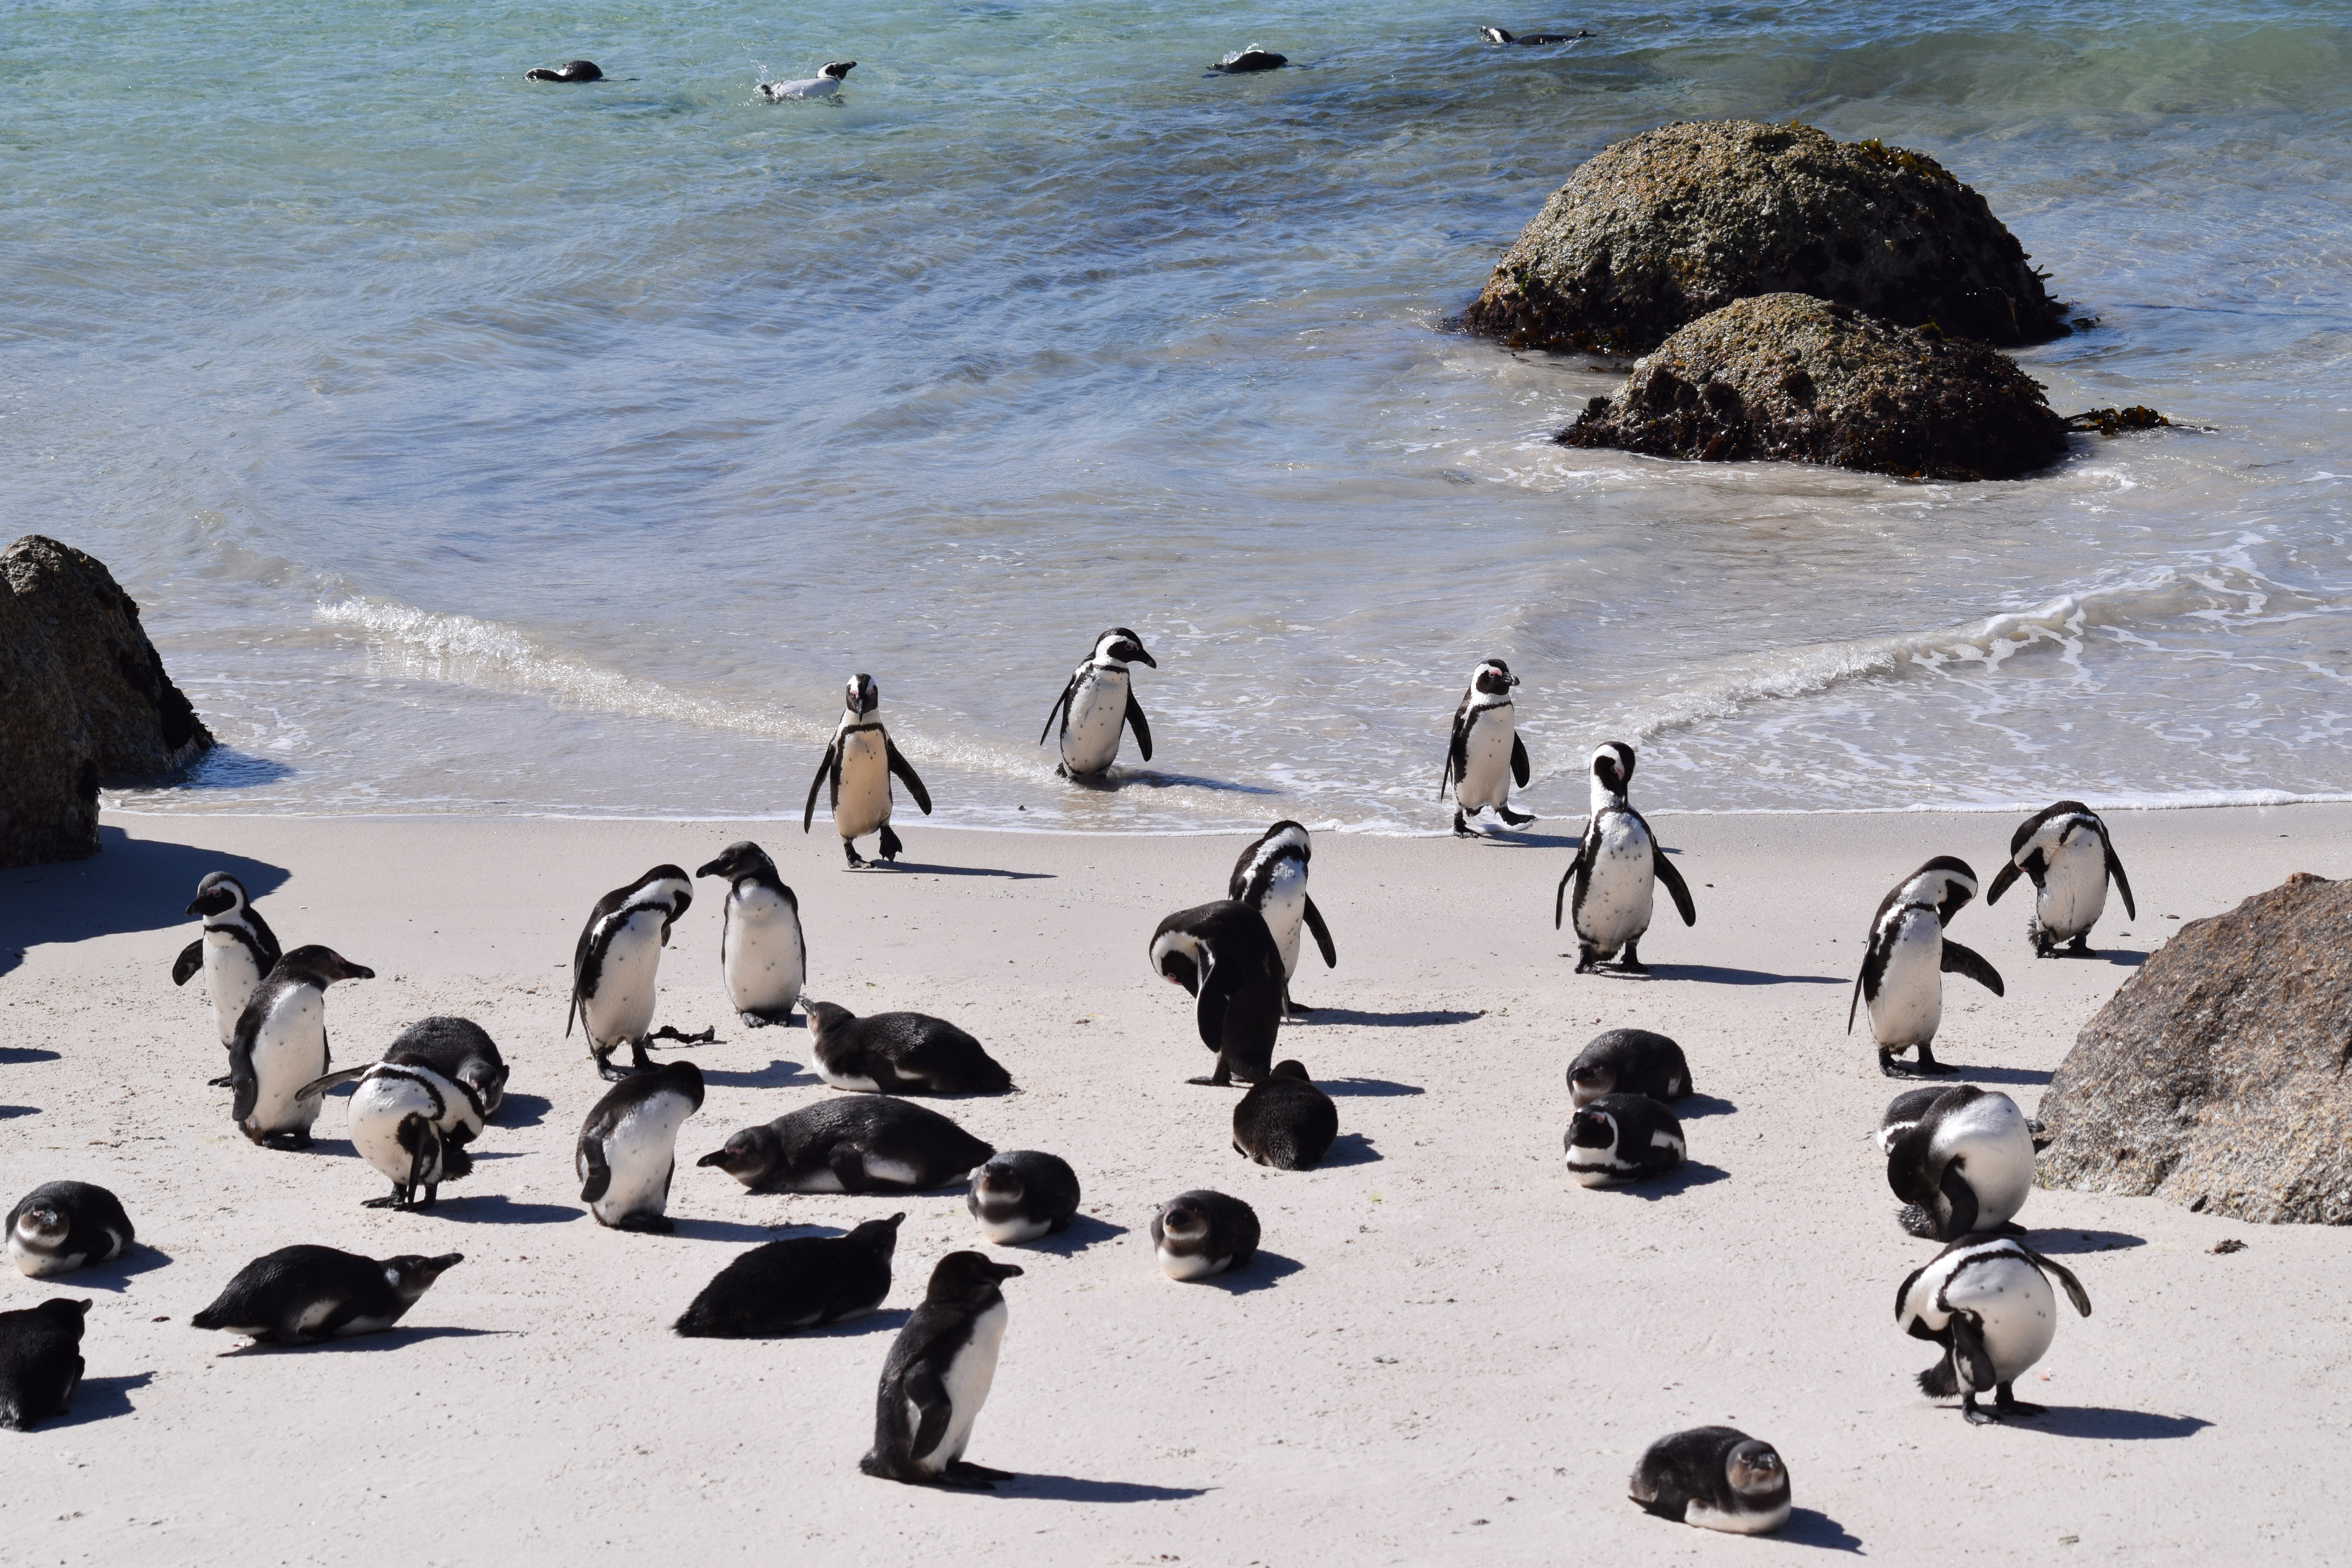
\includegraphics{../../images/posts/penguin-hero.jpg}

}

\caption{A penguin scientist with a magnifying glass, carefully
examining model diagnostics and residual plots!}

\end{figure}%

\emph{Photo: African penguins at Boulders Beach, South Africa. Licensed
under \href{https://creativecommons.org/licenses/by/2.0/}{CC BY 2.0} via
\href{https://commons.wikimedia.org/wiki/File:Boulders_Beach_penguins_(46475505885).jpg}{Wikimedia
Commons}}

\begin{tcolorbox}[enhanced jigsaw, breakable, opacityback=0, left=2mm, colback=white, bottomrule=.15mm, toprule=.15mm, arc=.35mm, rightrule=.15mm, leftrule=.75mm, colframe=quarto-callout-note-color-frame]
\begin{minipage}[t]{5.5mm}
\textcolor{quarto-callout-note-color}{\faInfo}
\end{minipage}%
\begin{minipage}[t]{\textwidth - 5.5mm}

\vspace{-3mm}\textbf{🐧 Palmer Penguins Data Analysis Series}\vspace{3mm}

This is \textbf{Part 4} of a 5-part series exploring penguin
morphometrics:

\begin{enumerate}
\def\labelenumi{\arabic{enumi}.}
\tightlist
\item
  \href{../palmer_penguins_part1/}{Part 1: EDA and Simple Regression}
\item
  \href{../palmer_penguins_part2/}{Part 2: Multiple Regression and
  Species Effects}
\item
  \href{../palmer_penguins_part3/}{Part 3: Advanced Models and
  Cross-Validation}
\item
  \textbf{Part 4: Model Diagnostics and Interpretation} (This post)
\item
  \href{../palmer_penguins_part5/}{Part 5: Random Forest vs Linear
  Models}
\end{enumerate}

\end{minipage}%
\end{tcolorbox}

\section{Introduction}\label{introduction}

Welcome to the fourth chapter of our Palmer penguins journey! In
\href{../palmer_penguins_part3/}{Part 3}, we validated our models
through rigorous cross-validation and confirmed that our species-aware
linear model offers excellent predictive performance. But excellent
performance doesn't automatically mean our model is appropriate or that
our assumptions are satisfied.

Today, we dive into the critical but often overlooked world of model
diagnostics. Think of this as taking your high-performing car to a
mechanic - it might run well, but are there underlying issues that could
cause problems? In statistical modeling, diagnostic procedures help us
understand whether our model is not just performing well, but performing
well for the right reasons.

In this post, we'll explore:

\begin{itemize}
\tightlist
\item
  Comprehensive residual analysis and assumption checking
\item
  Influence diagnostics to identify problematic observations
\item
  Biological interpretation of model coefficients
\item
  Prediction intervals and uncertainty quantification
\item
  Best practices for model reporting in ecological research
\end{itemize}

By the end of this post, you'll have confidence that your model is not
just accurate, but statistically sound and biologically meaningful.

\section{Setup and Model Preparation}\label{setup-and-model-preparation}

Let's reconstruct our best-performing model and prepare for diagnostic
analysis:

\begin{Shaded}
\begin{Highlighting}[]
\FunctionTok{library}\NormalTok{(palmerpenguins)}
\FunctionTok{library}\NormalTok{(tidyverse)}
\FunctionTok{library}\NormalTok{(broom)}
\CommentTok{\# Conditional loading of optional packages}
\NormalTok{optional\_diagnostic\_packages }\OtherTok{\textless{}{-}} \FunctionTok{c}\NormalTok{(}\StringTok{"car"}\NormalTok{, }\StringTok{"performance"}\NormalTok{, }\StringTok{"see"}\NormalTok{, }\StringTok{"lmtest"}\NormalTok{)}
\ControlFlowTok{for}\NormalTok{ (pkg }\ControlFlowTok{in}\NormalTok{ optional\_diagnostic\_packages) \{}
  \ControlFlowTok{if}\NormalTok{ (}\FunctionTok{requireNamespace}\NormalTok{(pkg, }\AttributeTok{quietly =} \ConstantTok{TRUE}\NormalTok{)) \{}
    \FunctionTok{library}\NormalTok{(pkg, }\AttributeTok{character.only =} \ConstantTok{TRUE}\NormalTok{)}
\NormalTok{  \} }\ControlFlowTok{else}\NormalTok{ \{}
    \FunctionTok{cat}\NormalTok{(}\StringTok{"⚠️ Package \textquotesingle{}"}\NormalTok{, pkg, }\StringTok{"\textquotesingle{} not available. Install with: install.packages(\textquotesingle{}"}\NormalTok{, pkg, }\StringTok{"\textquotesingle{})}\SpecialCharTok{\textbackslash{}n}\StringTok{"}\NormalTok{)}
\NormalTok{  \}}
\NormalTok{\}}
\FunctionTok{library}\NormalTok{(knitr)}
\FunctionTok{library}\NormalTok{(patchwork)}

\CommentTok{\# Set theme and colors}
\FunctionTok{theme\_set}\NormalTok{(}\FunctionTok{theme\_minimal}\NormalTok{(}\AttributeTok{base\_size =} \DecValTok{12}\NormalTok{))}
\NormalTok{penguin\_colors }\OtherTok{\textless{}{-}} \FunctionTok{c}\NormalTok{(}\StringTok{"Adelie"} \OtherTok{=} \StringTok{"\#FF6B6B"}\NormalTok{, }\StringTok{"Chinstrap"} \OtherTok{=} \StringTok{"\#4ECDC4"}\NormalTok{, }\StringTok{"Gentoo"} \OtherTok{=} \StringTok{"\#45B7D1"}\NormalTok{)}

\CommentTok{\# Load and prepare data}
\FunctionTok{data}\NormalTok{(penguins)}
\NormalTok{penguins\_clean }\OtherTok{\textless{}{-}}\NormalTok{ penguins }\SpecialCharTok{\%\textgreater{}\%} \FunctionTok{drop\_na}\NormalTok{()}

\CommentTok{\# Recreate our best model from previous parts}
\NormalTok{best\_model }\OtherTok{\textless{}{-}} \FunctionTok{lm}\NormalTok{(body\_mass\_g }\SpecialCharTok{\textasciitilde{}}\NormalTok{ bill\_length\_mm }\SpecialCharTok{+}\NormalTok{ bill\_depth\_mm }\SpecialCharTok{+} 
\NormalTok{                 flipper\_length\_mm }\SpecialCharTok{+}\NormalTok{ species, }\AttributeTok{data =}\NormalTok{ penguins\_clean)}

\CommentTok{\# Add fitted values and residuals to our dataset}
\NormalTok{penguins\_diagnostics }\OtherTok{\textless{}{-}}\NormalTok{ penguins\_clean }\SpecialCharTok{\%\textgreater{}\%}
  \FunctionTok{mutate}\NormalTok{(}
    \AttributeTok{fitted\_values =} \FunctionTok{fitted}\NormalTok{(best\_model),}
    \AttributeTok{residuals =} \FunctionTok{residuals}\NormalTok{(best\_model),}
    \AttributeTok{standardized\_residuals =} \FunctionTok{rstandard}\NormalTok{(best\_model),}
    \AttributeTok{studentized\_residuals =} \FunctionTok{rstudent}\NormalTok{(best\_model),}
    \AttributeTok{leverage =} \FunctionTok{hatvalues}\NormalTok{(best\_model),}
    \AttributeTok{cooks\_distance =} \FunctionTok{cooks.distance}\NormalTok{(best\_model)}
\NormalTok{  )}

\FunctionTok{cat}\NormalTok{(}\StringTok{"🔧 Model Diagnostic Setup:}\SpecialCharTok{\textbackslash{}n}\StringTok{"}\NormalTok{)}
\end{Highlighting}
\end{Shaded}

\begin{verbatim}
🔧 Model Diagnostic Setup:
\end{verbatim}

\begin{Shaded}
\begin{Highlighting}[]
\FunctionTok{cat}\NormalTok{(}\StringTok{"==========================}\SpecialCharTok{\textbackslash{}n}\StringTok{"}\NormalTok{)}
\end{Highlighting}
\end{Shaded}

\begin{verbatim}
==========================
\end{verbatim}

\begin{Shaded}
\begin{Highlighting}[]
\FunctionTok{cat}\NormalTok{(}\FunctionTok{sprintf}\NormalTok{(}\StringTok{"Model: body\_mass\_g \textasciitilde{} bill\_length\_mm + bill\_depth\_mm + flipper\_length\_mm + species}\SpecialCharTok{\textbackslash{}n}\StringTok{"}\NormalTok{))}
\end{Highlighting}
\end{Shaded}

\begin{verbatim}
Model: body_mass_g ~ bill_length_mm + bill_depth_mm + flipper_length_mm + species
\end{verbatim}

\begin{Shaded}
\begin{Highlighting}[]
\FunctionTok{cat}\NormalTok{(}\FunctionTok{sprintf}\NormalTok{(}\StringTok{"Observations: \%d}\SpecialCharTok{\textbackslash{}n}\StringTok{"}\NormalTok{, }\FunctionTok{nrow}\NormalTok{(penguins\_clean)))}
\end{Highlighting}
\end{Shaded}

\begin{verbatim}
Observations: 333
\end{verbatim}

\begin{Shaded}
\begin{Highlighting}[]
\FunctionTok{cat}\NormalTok{(}\FunctionTok{sprintf}\NormalTok{(}\StringTok{"Parameters: \%d}\SpecialCharTok{\textbackslash{}n}\StringTok{"}\NormalTok{, }\FunctionTok{length}\NormalTok{(}\FunctionTok{coef}\NormalTok{(best\_model))))}
\end{Highlighting}
\end{Shaded}

\begin{verbatim}
Parameters: 6
\end{verbatim}

\begin{Shaded}
\begin{Highlighting}[]
\FunctionTok{cat}\NormalTok{(}\FunctionTok{sprintf}\NormalTok{(}\StringTok{"R{-}squared: \%.3f}\SpecialCharTok{\textbackslash{}n}\StringTok{"}\NormalTok{, }\FunctionTok{summary}\NormalTok{(best\_model)}\SpecialCharTok{$}\NormalTok{r.squared))}
\end{Highlighting}
\end{Shaded}

\begin{verbatim}
R-squared: 0.849
\end{verbatim}

\section{Classical Regression
Assumptions}\label{classical-regression-assumptions}

Linear regression relies on several key assumptions. Let's check each
systematically:

\subsection{1. Linearity}\label{linearity}

The relationship between predictors and response should be linear:

\begin{Shaded}
\begin{Highlighting}[]
\CommentTok{\# Check linearity using partial residual plots}
\FunctionTok{par}\NormalTok{(}\AttributeTok{mfrow =} \FunctionTok{c}\NormalTok{(}\DecValTok{2}\NormalTok{, }\DecValTok{2}\NormalTok{))}
\FunctionTok{avPlots}\NormalTok{(best\_model, }\AttributeTok{main =} \StringTok{"Added{-}Variable Plots for Linearity"}\NormalTok{)}
\end{Highlighting}
\end{Shaded}

\includegraphics{index_files/figure-pdf/unnamed-chunk-2-1.pdf}

\begin{Shaded}
\begin{Highlighting}[]
\FunctionTok{par}\NormalTok{(}\AttributeTok{mfrow =} \FunctionTok{c}\NormalTok{(}\DecValTok{1}\NormalTok{, }\DecValTok{1}\NormalTok{))}

\CommentTok{\# Alternative: Component + residual plots}
\FunctionTok{crPlots}\NormalTok{(best\_model, }\AttributeTok{main =} \StringTok{"Component + Residual Plots"}\NormalTok{)}
\end{Highlighting}
\end{Shaded}

\includegraphics{index_files/figure-pdf/unnamed-chunk-2-2.pdf}

\begin{figure}[H]

{\centering \includegraphics{linearity-diagnostics.png}

}

\caption{Added-variable plots showing the linear relationships between
predictors and response after accounting for other variables}

\end{figure}%

\subsection{2. Independence of
Residuals}\label{independence-of-residuals}

We'll check for patterns that might indicate dependence:

\begin{Shaded}
\begin{Highlighting}[]
\CommentTok{\# Plot residuals vs order (temporal/spatial independence)}
\NormalTok{penguins\_diagnostics }\OtherTok{\textless{}{-}}\NormalTok{ penguins\_diagnostics }\SpecialCharTok{\%\textgreater{}\%}
  \FunctionTok{mutate}\NormalTok{(}\AttributeTok{observation\_order =} \FunctionTok{row\_number}\NormalTok{())}

\NormalTok{p1 }\OtherTok{\textless{}{-}} \FunctionTok{ggplot}\NormalTok{(penguins\_diagnostics, }\FunctionTok{aes}\NormalTok{(}\AttributeTok{x =}\NormalTok{ observation\_order, }\AttributeTok{y =}\NormalTok{ residuals)) }\SpecialCharTok{+}
  \FunctionTok{geom\_point}\NormalTok{(}\FunctionTok{aes}\NormalTok{(}\AttributeTok{color =}\NormalTok{ species), }\AttributeTok{alpha =} \FloatTok{0.7}\NormalTok{) }\SpecialCharTok{+}
  \FunctionTok{geom\_hline}\NormalTok{(}\AttributeTok{yintercept =} \DecValTok{0}\NormalTok{, }\AttributeTok{linetype =} \StringTok{"dashed"}\NormalTok{, }\AttributeTok{color =} \StringTok{"red"}\NormalTok{) }\SpecialCharTok{+}
  \FunctionTok{geom\_smooth}\NormalTok{(}\AttributeTok{method =} \StringTok{"loess"}\NormalTok{, }\AttributeTok{se =} \ConstantTok{TRUE}\NormalTok{, }\AttributeTok{color =} \StringTok{"blue"}\NormalTok{) }\SpecialCharTok{+}
  \FunctionTok{scale\_color\_manual}\NormalTok{(}\AttributeTok{values =}\NormalTok{ penguin\_colors) }\SpecialCharTok{+}
  \FunctionTok{labs}\NormalTok{(}\AttributeTok{title =} \StringTok{"Residuals vs Observation Order"}\NormalTok{,}
       \AttributeTok{subtitle =} \StringTok{"Checking for temporal/spatial patterns"}\NormalTok{,}
       \AttributeTok{x =} \StringTok{"Observation Order"}\NormalTok{, }\AttributeTok{y =} \StringTok{"Residuals (g)"}\NormalTok{,}
       \AttributeTok{color =} \StringTok{"Species"}\NormalTok{) }\SpecialCharTok{+}
  \FunctionTok{theme\_minimal}\NormalTok{()}

\FunctionTok{print}\NormalTok{(p1)}
\end{Highlighting}
\end{Shaded}

\includegraphics{index_files/figure-pdf/unnamed-chunk-3-1.pdf}

\begin{Shaded}
\begin{Highlighting}[]
\CommentTok{\# Durbin{-}Watson test for autocorrelation}
\NormalTok{dw\_test }\OtherTok{\textless{}{-}} \FunctionTok{durbinWatsonTest}\NormalTok{(best\_model)}
\FunctionTok{cat}\NormalTok{(}\StringTok{"}\SpecialCharTok{\textbackslash{}n}\StringTok{📊 Durbin{-}Watson Test for Autocorrelation:}\SpecialCharTok{\textbackslash{}n}\StringTok{"}\NormalTok{)}
\end{Highlighting}
\end{Shaded}

\begin{verbatim}

📊 Durbin-Watson Test for Autocorrelation:
\end{verbatim}

\begin{Shaded}
\begin{Highlighting}[]
\FunctionTok{cat}\NormalTok{(}\StringTok{"==========================================}\SpecialCharTok{\textbackslash{}n}\StringTok{"}\NormalTok{)}
\end{Highlighting}
\end{Shaded}

\begin{verbatim}
==========================================
\end{verbatim}

\begin{Shaded}
\begin{Highlighting}[]
\FunctionTok{cat}\NormalTok{(}\FunctionTok{sprintf}\NormalTok{(}\StringTok{"DW Statistic: \%.3f}\SpecialCharTok{\textbackslash{}n}\StringTok{"}\NormalTok{, dw\_test}\SpecialCharTok{$}\NormalTok{dw))}
\end{Highlighting}
\end{Shaded}

\begin{verbatim}
DW Statistic: 2.248
\end{verbatim}

\begin{Shaded}
\begin{Highlighting}[]
\FunctionTok{cat}\NormalTok{(}\FunctionTok{sprintf}\NormalTok{(}\StringTok{"p{-}value: \%.3f}\SpecialCharTok{\textbackslash{}n}\StringTok{"}\NormalTok{, dw\_test}\SpecialCharTok{$}\NormalTok{p))}
\end{Highlighting}
\end{Shaded}

\begin{verbatim}
p-value: 0.038
\end{verbatim}

\begin{Shaded}
\begin{Highlighting}[]
\FunctionTok{cat}\NormalTok{(}\StringTok{"Interpretation: Values near 2 indicate no autocorrelation}\SpecialCharTok{\textbackslash{}n}\StringTok{"}\NormalTok{)}
\end{Highlighting}
\end{Shaded}

\begin{verbatim}
Interpretation: Values near 2 indicate no autocorrelation
\end{verbatim}

\begin{figure}[H]

{\centering \includegraphics{independence-check.png}

}

\caption{Plot showing residuals versus observation order to check for
temporal or spatial dependencies}

\end{figure}%

\subsection{3. Homoscedasticity (Constant
Variance)}\label{homoscedasticity-constant-variance}

Residual variance should be constant across fitted values:

\begin{Shaded}
\begin{Highlighting}[]
\CommentTok{\# Residuals vs fitted values plot}
\NormalTok{p2 }\OtherTok{\textless{}{-}} \FunctionTok{ggplot}\NormalTok{(penguins\_diagnostics, }\FunctionTok{aes}\NormalTok{(}\AttributeTok{x =}\NormalTok{ fitted\_values, }\AttributeTok{y =}\NormalTok{ residuals)) }\SpecialCharTok{+}
  \FunctionTok{geom\_point}\NormalTok{(}\FunctionTok{aes}\NormalTok{(}\AttributeTok{color =}\NormalTok{ species), }\AttributeTok{alpha =} \FloatTok{0.7}\NormalTok{) }\SpecialCharTok{+}
  \FunctionTok{geom\_hline}\NormalTok{(}\AttributeTok{yintercept =} \DecValTok{0}\NormalTok{, }\AttributeTok{linetype =} \StringTok{"dashed"}\NormalTok{, }\AttributeTok{color =} \StringTok{"red"}\NormalTok{) }\SpecialCharTok{+}
  \FunctionTok{geom\_smooth}\NormalTok{(}\AttributeTok{method =} \StringTok{"loess"}\NormalTok{, }\AttributeTok{se =} \ConstantTok{TRUE}\NormalTok{, }\AttributeTok{color =} \StringTok{"blue"}\NormalTok{) }\SpecialCharTok{+}
  \FunctionTok{scale\_color\_manual}\NormalTok{(}\AttributeTok{values =}\NormalTok{ penguin\_colors) }\SpecialCharTok{+}
  \FunctionTok{labs}\NormalTok{(}\AttributeTok{title =} \StringTok{"Residuals vs Fitted Values"}\NormalTok{,}
       \AttributeTok{subtitle =} \StringTok{"Checking for homoscedasticity"}\NormalTok{,}
       \AttributeTok{x =} \StringTok{"Fitted Values (g)"}\NormalTok{, }\AttributeTok{y =} \StringTok{"Residuals (g)"}\NormalTok{,}
       \AttributeTok{color =} \StringTok{"Species"}\NormalTok{) }\SpecialCharTok{+}
  \FunctionTok{theme\_minimal}\NormalTok{()}

\CommentTok{\# Scale{-}Location plot (sqrt of absolute residuals)}
\NormalTok{p3 }\OtherTok{\textless{}{-}} \FunctionTok{ggplot}\NormalTok{(penguins\_diagnostics, }\FunctionTok{aes}\NormalTok{(}\AttributeTok{x =}\NormalTok{ fitted\_values, }\AttributeTok{y =} \FunctionTok{sqrt}\NormalTok{(}\FunctionTok{abs}\NormalTok{(residuals)))) }\SpecialCharTok{+}
  \FunctionTok{geom\_point}\NormalTok{(}\FunctionTok{aes}\NormalTok{(}\AttributeTok{color =}\NormalTok{ species), }\AttributeTok{alpha =} \FloatTok{0.7}\NormalTok{) }\SpecialCharTok{+}
  \FunctionTok{geom\_smooth}\NormalTok{(}\AttributeTok{method =} \StringTok{"loess"}\NormalTok{, }\AttributeTok{se =} \ConstantTok{TRUE}\NormalTok{, }\AttributeTok{color =} \StringTok{"blue"}\NormalTok{) }\SpecialCharTok{+}
  \FunctionTok{scale\_color\_manual}\NormalTok{(}\AttributeTok{values =}\NormalTok{ penguin\_colors) }\SpecialCharTok{+}
  \FunctionTok{labs}\NormalTok{(}\AttributeTok{title =} \StringTok{"Scale{-}Location Plot"}\NormalTok{,}
       \AttributeTok{subtitle =} \StringTok{"Square root of absolute residuals vs fitted values"}\NormalTok{,}
       \AttributeTok{x =} \StringTok{"Fitted Values (g)"}\NormalTok{, }\AttributeTok{y =} \StringTok{"√|Residuals|"}\NormalTok{,}
       \AttributeTok{color =} \StringTok{"Species"}\NormalTok{) }\SpecialCharTok{+}
  \FunctionTok{theme\_minimal}\NormalTok{()}

\NormalTok{homoscedasticity\_plots }\OtherTok{\textless{}{-}}\NormalTok{ p2 }\SpecialCharTok{+}\NormalTok{ p3}
\FunctionTok{print}\NormalTok{(homoscedasticity\_plots)}
\end{Highlighting}
\end{Shaded}

\includegraphics{index_files/figure-pdf/unnamed-chunk-4-1.pdf}

\begin{Shaded}
\begin{Highlighting}[]
\CommentTok{\# Breusch{-}Pagan test for heteroscedasticity}
\NormalTok{bp\_test }\OtherTok{\textless{}{-}} \FunctionTok{bptest}\NormalTok{(best\_model)}
\FunctionTok{cat}\NormalTok{(}\StringTok{"}\SpecialCharTok{\textbackslash{}n}\StringTok{📊 Breusch{-}Pagan Test for Heteroscedasticity:}\SpecialCharTok{\textbackslash{}n}\StringTok{"}\NormalTok{)}
\end{Highlighting}
\end{Shaded}

\begin{verbatim}

📊 Breusch-Pagan Test for Heteroscedasticity:
\end{verbatim}

\begin{Shaded}
\begin{Highlighting}[]
\FunctionTok{cat}\NormalTok{(}\StringTok{"==============================================}\SpecialCharTok{\textbackslash{}n}\StringTok{"}\NormalTok{)}
\end{Highlighting}
\end{Shaded}

\begin{verbatim}
==============================================
\end{verbatim}

\begin{Shaded}
\begin{Highlighting}[]
\FunctionTok{cat}\NormalTok{(}\FunctionTok{sprintf}\NormalTok{(}\StringTok{"BP Statistic: \%.3f}\SpecialCharTok{\textbackslash{}n}\StringTok{"}\NormalTok{, bp\_test}\SpecialCharTok{$}\NormalTok{statistic))}
\end{Highlighting}
\end{Shaded}

\begin{verbatim}
BP Statistic: 2.583
\end{verbatim}

\begin{Shaded}
\begin{Highlighting}[]
\FunctionTok{cat}\NormalTok{(}\FunctionTok{sprintf}\NormalTok{(}\StringTok{"p{-}value: \%.3f}\SpecialCharTok{\textbackslash{}n}\StringTok{"}\NormalTok{, bp\_test}\SpecialCharTok{$}\NormalTok{p.value))}
\end{Highlighting}
\end{Shaded}

\begin{verbatim}
p-value: 0.764
\end{verbatim}

\begin{Shaded}
\begin{Highlighting}[]
\FunctionTok{cat}\NormalTok{(}\StringTok{"Interpretation: p \textgreater{} 0.05 suggests constant variance (homoscedasticity)}\SpecialCharTok{\textbackslash{}n}\StringTok{"}\NormalTok{)}
\end{Highlighting}
\end{Shaded}

\begin{verbatim}
Interpretation: p > 0.05 suggests constant variance (homoscedasticity)
\end{verbatim}

\begin{figure}[H]

{\centering \includegraphics{homoscedasticity-diagnostics.png}

}

\caption{Diagnostic plots for checking homoscedasticity assumption
through residuals vs fitted values}

\end{figure}%

\subsection{4. Normality of Residuals}\label{normality-of-residuals}

Residuals should follow a normal distribution:

\begin{Shaded}
\begin{Highlighting}[]
\CommentTok{\# Q{-}Q plot for normality}
\NormalTok{p4 }\OtherTok{\textless{}{-}} \FunctionTok{ggplot}\NormalTok{(penguins\_diagnostics, }\FunctionTok{aes}\NormalTok{(}\AttributeTok{sample =}\NormalTok{ standardized\_residuals)) }\SpecialCharTok{+}
  \FunctionTok{stat\_qq}\NormalTok{(}\FunctionTok{aes}\NormalTok{(}\AttributeTok{color =}\NormalTok{ species), }\AttributeTok{alpha =} \FloatTok{0.7}\NormalTok{) }\SpecialCharTok{+}
  \FunctionTok{stat\_qq\_line}\NormalTok{(}\AttributeTok{color =} \StringTok{"red"}\NormalTok{, }\AttributeTok{linetype =} \StringTok{"dashed"}\NormalTok{) }\SpecialCharTok{+}
  \FunctionTok{scale\_color\_manual}\NormalTok{(}\AttributeTok{values =}\NormalTok{ penguin\_colors) }\SpecialCharTok{+}
  \FunctionTok{labs}\NormalTok{(}\AttributeTok{title =} \StringTok{"Q{-}Q Plot of Standardized Residuals"}\NormalTok{,}
       \AttributeTok{subtitle =} \StringTok{"Checking normality assumption"}\NormalTok{,}
       \AttributeTok{x =} \StringTok{"Theoretical Quantiles"}\NormalTok{, }\AttributeTok{y =} \StringTok{"Sample Quantiles"}\NormalTok{,}
       \AttributeTok{color =} \StringTok{"Species"}\NormalTok{) }\SpecialCharTok{+}
  \FunctionTok{theme\_minimal}\NormalTok{()}

\CommentTok{\# Histogram of residuals}
\NormalTok{p5 }\OtherTok{\textless{}{-}} \FunctionTok{ggplot}\NormalTok{(penguins\_diagnostics, }\FunctionTok{aes}\NormalTok{(}\AttributeTok{x =}\NormalTok{ residuals)) }\SpecialCharTok{+}
  \FunctionTok{geom\_histogram}\NormalTok{(}\FunctionTok{aes}\NormalTok{(}\AttributeTok{y =} \FunctionTok{after\_stat}\NormalTok{(density)), }\AttributeTok{bins =} \DecValTok{30}\NormalTok{, }
                 \AttributeTok{fill =} \StringTok{"lightblue"}\NormalTok{, }\AttributeTok{alpha =} \FloatTok{0.7}\NormalTok{, }\AttributeTok{color =} \StringTok{"white"}\NormalTok{) }\SpecialCharTok{+}
  \FunctionTok{geom\_density}\NormalTok{(}\AttributeTok{color =} \StringTok{"blue"}\NormalTok{, }\AttributeTok{size =} \DecValTok{1}\NormalTok{) }\SpecialCharTok{+}
  \FunctionTok{stat\_function}\NormalTok{(}\AttributeTok{fun =}\NormalTok{ dnorm, }
                \AttributeTok{args =} \FunctionTok{list}\NormalTok{(}\AttributeTok{mean =} \FunctionTok{mean}\NormalTok{(penguins\_diagnostics}\SpecialCharTok{$}\NormalTok{residuals), }
                           \AttributeTok{sd =} \FunctionTok{sd}\NormalTok{(penguins\_diagnostics}\SpecialCharTok{$}\NormalTok{residuals)),}
                \AttributeTok{color =} \StringTok{"red"}\NormalTok{, }\AttributeTok{linetype =} \StringTok{"dashed"}\NormalTok{, }\AttributeTok{size =} \DecValTok{1}\NormalTok{) }\SpecialCharTok{+}
  \FunctionTok{labs}\NormalTok{(}\AttributeTok{title =} \StringTok{"Distribution of Residuals"}\NormalTok{,}
       \AttributeTok{subtitle =} \StringTok{"Blue = actual density, Red = normal distribution"}\NormalTok{,}
       \AttributeTok{x =} \StringTok{"Residuals (g)"}\NormalTok{, }\AttributeTok{y =} \StringTok{"Density"}\NormalTok{) }\SpecialCharTok{+}
  \FunctionTok{theme\_minimal}\NormalTok{()}

\NormalTok{normality\_plots }\OtherTok{\textless{}{-}}\NormalTok{ p4 }\SpecialCharTok{+}\NormalTok{ p5}
\FunctionTok{print}\NormalTok{(normality\_plots)}
\end{Highlighting}
\end{Shaded}

\includegraphics{index_files/figure-pdf/unnamed-chunk-5-1.pdf}

\begin{Shaded}
\begin{Highlighting}[]
\CommentTok{\# Shapiro{-}Wilk test for normality}
\NormalTok{shapiro\_test }\OtherTok{\textless{}{-}} \FunctionTok{shapiro.test}\NormalTok{(}\FunctionTok{residuals}\NormalTok{(best\_model))}
\FunctionTok{cat}\NormalTok{(}\StringTok{"}\SpecialCharTok{\textbackslash{}n}\StringTok{📊 Shapiro{-}Wilk Test for Normality:}\SpecialCharTok{\textbackslash{}n}\StringTok{"}\NormalTok{)}
\end{Highlighting}
\end{Shaded}

\begin{verbatim}

📊 Shapiro-Wilk Test for Normality:
\end{verbatim}

\begin{Shaded}
\begin{Highlighting}[]
\FunctionTok{cat}\NormalTok{(}\StringTok{"====================================}\SpecialCharTok{\textbackslash{}n}\StringTok{"}\NormalTok{)}
\end{Highlighting}
\end{Shaded}

\begin{verbatim}
====================================
\end{verbatim}

\begin{Shaded}
\begin{Highlighting}[]
\FunctionTok{cat}\NormalTok{(}\FunctionTok{sprintf}\NormalTok{(}\StringTok{"W Statistic: \%.4f}\SpecialCharTok{\textbackslash{}n}\StringTok{"}\NormalTok{, shapiro\_test}\SpecialCharTok{$}\NormalTok{statistic))}
\end{Highlighting}
\end{Shaded}

\begin{verbatim}
W Statistic: 0.9921
\end{verbatim}

\begin{Shaded}
\begin{Highlighting}[]
\FunctionTok{cat}\NormalTok{(}\FunctionTok{sprintf}\NormalTok{(}\StringTok{"p{-}value: \%.4f}\SpecialCharTok{\textbackslash{}n}\StringTok{"}\NormalTok{, shapiro\_test}\SpecialCharTok{$}\NormalTok{p.value))}
\end{Highlighting}
\end{Shaded}

\begin{verbatim}
p-value: 0.0746
\end{verbatim}

\begin{Shaded}
\begin{Highlighting}[]
\FunctionTok{cat}\NormalTok{(}\StringTok{"Interpretation: p \textgreater{} 0.05 suggests residuals are normally distributed}\SpecialCharTok{\textbackslash{}n}\StringTok{"}\NormalTok{)}
\end{Highlighting}
\end{Shaded}

\begin{verbatim}
Interpretation: p > 0.05 suggests residuals are normally distributed
\end{verbatim}

\begin{Shaded}
\begin{Highlighting}[]
\CommentTok{\# Alternative: Anderson{-}Darling test (more powerful for large samples)}
\CommentTok{\# Install nortest if needed: install.packages("nortest")}
\ControlFlowTok{if}\NormalTok{ (}\FunctionTok{requireNamespace}\NormalTok{(}\StringTok{"nortest"}\NormalTok{, }\AttributeTok{quietly =} \ConstantTok{TRUE}\NormalTok{)) \{}
  \FunctionTok{library}\NormalTok{(nortest)}
\NormalTok{  ad\_test }\OtherTok{\textless{}{-}} \FunctionTok{ad.test}\NormalTok{(}\FunctionTok{residuals}\NormalTok{(best\_model))}
  \FunctionTok{cat}\NormalTok{(}\FunctionTok{sprintf}\NormalTok{(}\StringTok{"}\SpecialCharTok{\textbackslash{}n}\StringTok{Anderson{-}Darling Test p{-}value: \%.4f}\SpecialCharTok{\textbackslash{}n}\StringTok{"}\NormalTok{, ad\_test}\SpecialCharTok{$}\NormalTok{p.value))}
\NormalTok{\} }\ControlFlowTok{else}\NormalTok{ \{}
  \FunctionTok{cat}\NormalTok{(}\StringTok{"}\SpecialCharTok{\textbackslash{}n}\StringTok{⚠️ nortest package not available. Install with: install.packages(\textquotesingle{}nortest\textquotesingle{})}\SpecialCharTok{\textbackslash{}n}\StringTok{"}\NormalTok{)}
  \FunctionTok{cat}\NormalTok{(}\StringTok{"Using Shapiro{-}Wilk test results instead.}\SpecialCharTok{\textbackslash{}n}\StringTok{"}\NormalTok{)}
\NormalTok{\}}
\end{Highlighting}
\end{Shaded}

\begin{verbatim}

⚠️ nortest package not available. Install with: install.packages('nortest')
Using Shapiro-Wilk test results instead.
\end{verbatim}

\begin{figure}[H]

{\centering \includegraphics{normality-diagnostics.png}

}

\caption{Diagnostic plots for checking normality of residuals including
Q-Q plot and histogram}

\end{figure}%

\section{Influence Diagnostics}\label{influence-diagnostics}

Some observations might have disproportionate influence on our model.
Let's identify them:

\subsection{Leverage, Outliers, and Influential
Points}\label{leverage-outliers-and-influential-points}

\begin{Shaded}
\begin{Highlighting}[]
\CommentTok{\# Calculate diagnostic thresholds}
\NormalTok{n }\OtherTok{\textless{}{-}} \FunctionTok{nrow}\NormalTok{(penguins\_clean)}
\NormalTok{p }\OtherTok{\textless{}{-}} \FunctionTok{length}\NormalTok{(}\FunctionTok{coef}\NormalTok{(best\_model))}

\CommentTok{\# Thresholds}
\NormalTok{leverage\_threshold }\OtherTok{\textless{}{-}} \DecValTok{2} \SpecialCharTok{*}\NormalTok{ p }\SpecialCharTok{/}\NormalTok{ n}
\NormalTok{cooks\_threshold }\OtherTok{\textless{}{-}} \DecValTok{4} \SpecialCharTok{/}\NormalTok{ n}
\NormalTok{studentized\_threshold }\OtherTok{\textless{}{-}} \FunctionTok{qt}\NormalTok{(}\FloatTok{0.975}\NormalTok{, n }\SpecialCharTok{{-}}\NormalTok{ p }\SpecialCharTok{{-}} \DecValTok{1}\NormalTok{)  }\CommentTok{\# Two{-}tailed 95\%}

\FunctionTok{cat}\NormalTok{(}\StringTok{"🎯 Diagnostic Thresholds:}\SpecialCharTok{\textbackslash{}n}\StringTok{"}\NormalTok{)}
\end{Highlighting}
\end{Shaded}

\begin{verbatim}
🎯 Diagnostic Thresholds:
\end{verbatim}

\begin{Shaded}
\begin{Highlighting}[]
\FunctionTok{cat}\NormalTok{(}\StringTok{"=========================}\SpecialCharTok{\textbackslash{}n}\StringTok{"}\NormalTok{)}
\end{Highlighting}
\end{Shaded}

\begin{verbatim}
=========================
\end{verbatim}

\begin{Shaded}
\begin{Highlighting}[]
\FunctionTok{cat}\NormalTok{(}\FunctionTok{sprintf}\NormalTok{(}\StringTok{"High leverage threshold: \%.3f}\SpecialCharTok{\textbackslash{}n}\StringTok{"}\NormalTok{, leverage\_threshold))}
\end{Highlighting}
\end{Shaded}

\begin{verbatim}
High leverage threshold: 0.036
\end{verbatim}

\begin{Shaded}
\begin{Highlighting}[]
\FunctionTok{cat}\NormalTok{(}\FunctionTok{sprintf}\NormalTok{(}\StringTok{"High Cook\textquotesingle{}s distance threshold: \%.3f}\SpecialCharTok{\textbackslash{}n}\StringTok{"}\NormalTok{, cooks\_threshold))}
\end{Highlighting}
\end{Shaded}

\begin{verbatim}
High Cook's distance threshold: 0.012
\end{verbatim}

\begin{Shaded}
\begin{Highlighting}[]
\FunctionTok{cat}\NormalTok{(}\FunctionTok{sprintf}\NormalTok{(}\StringTok{"Studentized residual threshold: ±\%.2f}\SpecialCharTok{\textbackslash{}n}\StringTok{"}\NormalTok{, studentized\_threshold))}
\end{Highlighting}
\end{Shaded}

\begin{verbatim}
Studentized residual threshold: ±1.97
\end{verbatim}

\begin{Shaded}
\begin{Highlighting}[]
\CommentTok{\# Identify problematic observations}
\NormalTok{problematic\_obs }\OtherTok{\textless{}{-}}\NormalTok{ penguins\_diagnostics }\SpecialCharTok{\%\textgreater{}\%}
  \FunctionTok{mutate}\NormalTok{(}
    \AttributeTok{high\_leverage =}\NormalTok{ leverage }\SpecialCharTok{\textgreater{}}\NormalTok{ leverage\_threshold,}
    \AttributeTok{high\_cooks =}\NormalTok{ cooks\_distance }\SpecialCharTok{\textgreater{}}\NormalTok{ cooks\_threshold,}
    \AttributeTok{outlier =} \FunctionTok{abs}\NormalTok{(studentized\_residuals) }\SpecialCharTok{\textgreater{}}\NormalTok{ studentized\_threshold,}
    \AttributeTok{influential =}\NormalTok{ high\_leverage }\SpecialCharTok{|}\NormalTok{ high\_cooks }\SpecialCharTok{|}\NormalTok{ outlier,}
    \AttributeTok{obs\_id =} \FunctionTok{row\_number}\NormalTok{()}
\NormalTok{  ) }\SpecialCharTok{\%\textgreater{}\%}
  \FunctionTok{filter}\NormalTok{(influential)}

\FunctionTok{cat}\NormalTok{(}\FunctionTok{sprintf}\NormalTok{(}\StringTok{"}\SpecialCharTok{\textbackslash{}n}\StringTok{🔍 Identified \%d potentially problematic observations:}\SpecialCharTok{\textbackslash{}n}\StringTok{"}\NormalTok{, }\FunctionTok{nrow}\NormalTok{(problematic\_obs)))}
\end{Highlighting}
\end{Shaded}

\begin{verbatim}

🔍 Identified 30 potentially problematic observations:
\end{verbatim}

\begin{Shaded}
\begin{Highlighting}[]
\FunctionTok{cat}\NormalTok{(}\StringTok{"==============================================}\SpecialCharTok{\textbackslash{}n}\StringTok{"}\NormalTok{)}
\end{Highlighting}
\end{Shaded}

\begin{verbatim}
==============================================
\end{verbatim}

\begin{Shaded}
\begin{Highlighting}[]
\ControlFlowTok{if}\NormalTok{(}\FunctionTok{nrow}\NormalTok{(problematic\_obs) }\SpecialCharTok{\textgreater{}} \DecValTok{0}\NormalTok{) \{}
\NormalTok{  problematic\_summary }\OtherTok{\textless{}{-}}\NormalTok{ problematic\_obs }\SpecialCharTok{\%\textgreater{}\%}
    \FunctionTok{select}\NormalTok{(obs\_id, species, body\_mass\_g, fitted\_values, leverage, }
\NormalTok{           cooks\_distance, studentized\_residuals, high\_leverage, high\_cooks, outlier)}
  
  \FunctionTok{print}\NormalTok{(}\FunctionTok{kable}\NormalTok{(problematic\_summary, }\AttributeTok{digits =} \DecValTok{3}\NormalTok{,}
              \AttributeTok{caption =} \StringTok{"Potentially Influential Observations"}\NormalTok{))}
\NormalTok{\}}
\end{Highlighting}
\end{Shaded}

\begin{verbatim}


Table: Potentially Influential Observations

| obs_id|species   | body_mass_g| fitted_values| leverage| cooks_distance| studentized_residuals|high_leverage |high_cooks |outlier |
|------:|:---------|-----------:|-------------:|--------:|--------------:|---------------------:|:-------------|:----------|:-------|
|      7|Adelie    |        4675|      3997.756|    0.012|          0.009|                 2.177|FALSE         |FALSE      |TRUE    |
|      9|Adelie    |        3800|      4119.854|    0.037|          0.007|                -1.036|TRUE          |FALSE      |FALSE   |
|     10|Adelie    |        4400|      4088.388|    0.059|          0.011|                 1.021|TRUE          |FALSE      |FALSE   |
|     15|Adelie    |        4200|      4516.981|    0.040|          0.007|                -1.028|TRUE          |FALSE      |FALSE   |
|     24|Adelie    |        3150|      3339.143|    0.040|          0.003|                -0.613|TRUE          |FALSE      |FALSE   |
|     35|Adelie    |        4650|      3728.211|    0.015|          0.022|                 2.986|FALSE         |TRUE       |TRUE    |
|     41|Adelie    |        4600|      3799.094|    0.008|          0.008|                 2.576|FALSE         |FALSE      |TRUE    |
|     76|Adelie    |        4700|      3881.398|    0.023|          0.027|                 2.655|FALSE         |TRUE       |TRUE    |
|     88|Adelie    |        4450|      3618.949|    0.009|          0.011|                 2.678|FALSE         |FALSE      |TRUE    |
|     99|Adelie    |        2925|      3763.898|    0.009|          0.010|                -2.703|FALSE         |FALSE      |TRUE    |
|    104|Adelie    |        4775|      4112.020|    0.014|          0.011|                 2.133|FALSE         |FALSE      |TRUE    |
|    124|Adelie    |        4000|      4268.939|    0.051|          0.007|                -0.877|TRUE          |FALSE      |FALSE   |
|    126|Adelie    |        3500|      4136.402|    0.014|          0.010|                -2.046|FALSE         |FALSE      |TRUE    |
|    128|Adelie    |        4475|      3855.192|    0.017|          0.011|                 1.995|FALSE         |FALSE      |TRUE    |
|    137|Adelie    |        3050|      2992.908|    0.036|          0.000|                 0.185|TRUE          |FALSE      |FALSE   |
|    160|Gentoo    |        5850|      4983.583|    0.011|          0.015|                 2.797|FALSE         |TRUE       |TRUE    |
|    161|Gentoo    |        4200|      4819.636|    0.012|          0.008|                -1.990|FALSE         |FALSE      |TRUE    |
|    164|Gentoo    |        6300|      5262.232|    0.010|          0.018|                 3.365|FALSE         |TRUE       |TRUE    |
|    179|Gentoo    |        6050|      6112.530|    0.059|          0.000|                -0.204|TRUE          |FALSE      |FALSE   |
|    183|Gentoo    |        5250|      5328.851|    0.041|          0.000|                -0.255|TRUE          |FALSE      |FALSE   |
|    224|Gentoo    |        5950|      5313.937|    0.024|          0.017|                 2.056|FALSE         |TRUE       |TRUE    |
|    272|Chinstrap |        3250|      3232.725|    0.041|          0.000|                 0.056|TRUE          |FALSE      |FALSE   |
|    282|Chinstrap |        3300|      4039.034|    0.022|          0.021|                -2.391|FALSE         |TRUE       |TRUE    |
|    283|Chinstrap |        3700|      3709.345|    0.104|          0.000|                -0.031|TRUE          |FALSE      |FALSE   |
|    285|Chinstrap |        4400|      3699.702|    0.015|          0.013|                 2.256|FALSE         |TRUE       |TRUE    |
|    286|Chinstrap |        3600|      3018.853|    0.036|          0.022|                 1.887|FALSE         |TRUE       |FALSE   |
|    296|Chinstrap |        3200|      2981.394|    0.036|          0.003|                 0.707|TRUE          |FALSE      |FALSE   |
|    304|Chinstrap |        2700|      3320.836|    0.023|          0.016|                -2.005|FALSE         |TRUE       |TRUE    |
|    313|Chinstrap |        4300|      4234.088|    0.038|          0.000|                 0.213|TRUE          |FALSE      |FALSE   |
|    330|Chinstrap |        3400|      3600.715|    0.037|          0.003|                -0.649|TRUE          |FALSE      |FALSE   |
\end{verbatim}

\subsection{Influence Plot}\label{influence-plot}

\begin{Shaded}
\begin{Highlighting}[]
\CommentTok{\# Create comprehensive influence plot}
\NormalTok{p6 }\OtherTok{\textless{}{-}} \FunctionTok{ggplot}\NormalTok{(penguins\_diagnostics, }\FunctionTok{aes}\NormalTok{(}\AttributeTok{x =}\NormalTok{ leverage, }\AttributeTok{y =} \FunctionTok{abs}\NormalTok{(studentized\_residuals))) }\SpecialCharTok{+}
  \FunctionTok{geom\_point}\NormalTok{(}\FunctionTok{aes}\NormalTok{(}\AttributeTok{size =}\NormalTok{ cooks\_distance, }\AttributeTok{color =}\NormalTok{ species), }\AttributeTok{alpha =} \FloatTok{0.7}\NormalTok{) }\SpecialCharTok{+}
  \FunctionTok{geom\_hline}\NormalTok{(}\AttributeTok{yintercept =}\NormalTok{ studentized\_threshold, }\AttributeTok{linetype =} \StringTok{"dashed"}\NormalTok{, }\AttributeTok{color =} \StringTok{"red"}\NormalTok{) }\SpecialCharTok{+}
  \FunctionTok{geom\_vline}\NormalTok{(}\AttributeTok{xintercept =}\NormalTok{ leverage\_threshold, }\AttributeTok{linetype =} \StringTok{"dashed"}\NormalTok{, }\AttributeTok{color =} \StringTok{"red"}\NormalTok{) }\SpecialCharTok{+}
  \FunctionTok{scale\_color\_manual}\NormalTok{(}\AttributeTok{values =}\NormalTok{ penguin\_colors) }\SpecialCharTok{+}
  \FunctionTok{scale\_size\_continuous}\NormalTok{(}\AttributeTok{range =} \FunctionTok{c}\NormalTok{(}\DecValTok{1}\NormalTok{, }\DecValTok{4}\NormalTok{), }\AttributeTok{name =} \StringTok{"Cook\textquotesingle{}s D"}\NormalTok{) }\SpecialCharTok{+}
  \FunctionTok{labs}\NormalTok{(}\AttributeTok{title =} \StringTok{"Influence Plot"}\NormalTok{,}
       \AttributeTok{subtitle =} \StringTok{"Size = Cook\textquotesingle{}s distance, Lines = thresholds"}\NormalTok{,}
       \AttributeTok{x =} \StringTok{"Leverage"}\NormalTok{, }\AttributeTok{y =} \StringTok{"|Studentized Residuals|"}\NormalTok{,}
       \AttributeTok{color =} \StringTok{"Species"}\NormalTok{) }\SpecialCharTok{+}
  \FunctionTok{theme\_minimal}\NormalTok{()}

\CommentTok{\# Cook\textquotesingle{}s distance plot}
\NormalTok{p7 }\OtherTok{\textless{}{-}} \FunctionTok{ggplot}\NormalTok{(penguins\_diagnostics, }\FunctionTok{aes}\NormalTok{(}\AttributeTok{x =}\NormalTok{ observation\_order, }\AttributeTok{y =}\NormalTok{ cooks\_distance)) }\SpecialCharTok{+}
  \FunctionTok{geom\_col}\NormalTok{(}\FunctionTok{aes}\NormalTok{(}\AttributeTok{fill =}\NormalTok{ species), }\AttributeTok{alpha =} \FloatTok{0.7}\NormalTok{) }\SpecialCharTok{+}
  \FunctionTok{geom\_hline}\NormalTok{(}\AttributeTok{yintercept =}\NormalTok{ cooks\_threshold, }\AttributeTok{linetype =} \StringTok{"dashed"}\NormalTok{, }\AttributeTok{color =} \StringTok{"red"}\NormalTok{) }\SpecialCharTok{+}
  \FunctionTok{scale\_fill\_manual}\NormalTok{(}\AttributeTok{values =}\NormalTok{ penguin\_colors) }\SpecialCharTok{+}
  \FunctionTok{labs}\NormalTok{(}\AttributeTok{title =} \StringTok{"Cook\textquotesingle{}s Distance by Observation"}\NormalTok{,}
       \AttributeTok{subtitle =} \StringTok{"Red line shows threshold for high influence"}\NormalTok{,}
       \AttributeTok{x =} \StringTok{"Observation Number"}\NormalTok{, }\AttributeTok{y =} \StringTok{"Cook\textquotesingle{}s Distance"}\NormalTok{,}
       \AttributeTok{fill =} \StringTok{"Species"}\NormalTok{) }\SpecialCharTok{+}
  \FunctionTok{theme\_minimal}\NormalTok{()}

\NormalTok{influence\_plots }\OtherTok{\textless{}{-}}\NormalTok{ p6 }\SpecialCharTok{+}\NormalTok{ p7}
\FunctionTok{print}\NormalTok{(influence\_plots)}
\end{Highlighting}
\end{Shaded}

\includegraphics{index_files/figure-pdf/unnamed-chunk-7-1.pdf}

\begin{figure}[H]

{\centering \includegraphics{influence-diagnostics.png}

}

\caption{Influence diagnostic plots showing leverage, Cook's distance,
and studentized residuals}

\end{figure}%

\section{Model Performance
Diagnostics}\label{model-performance-diagnostics}

Let's use the performance package for additional diagnostics:

\begin{Shaded}
\begin{Highlighting}[]
\CommentTok{\# Comprehensive model check}
\NormalTok{model\_performance }\OtherTok{\textless{}{-}} \FunctionTok{check\_model}\NormalTok{(best\_model)}
\FunctionTok{plot}\NormalTok{(model\_performance)}
\end{Highlighting}
\end{Shaded}

\includegraphics{index_files/figure-pdf/unnamed-chunk-8-1.pdf}

\begin{Shaded}
\begin{Highlighting}[]
\CommentTok{\# Individual performance metrics}
\FunctionTok{cat}\NormalTok{(}\StringTok{"}\SpecialCharTok{\textbackslash{}n}\StringTok{📈 Model Performance Summary:}\SpecialCharTok{\textbackslash{}n}\StringTok{"}\NormalTok{)}
\end{Highlighting}
\end{Shaded}

\begin{verbatim}

📈 Model Performance Summary:
\end{verbatim}

\begin{Shaded}
\begin{Highlighting}[]
\FunctionTok{cat}\NormalTok{(}\StringTok{"=============================}\SpecialCharTok{\textbackslash{}n}\StringTok{"}\NormalTok{)}
\end{Highlighting}
\end{Shaded}

\begin{verbatim}
=============================
\end{verbatim}

\begin{Shaded}
\begin{Highlighting}[]
\CommentTok{\# Model performance indices}
\NormalTok{perf\_metrics }\OtherTok{\textless{}{-}} \FunctionTok{model\_performance}\NormalTok{(best\_model)}
\FunctionTok{print}\NormalTok{(perf\_metrics)}
\end{Highlighting}
\end{Shaded}

\begin{verbatim}
# Indices of model performance

AIC      |     AICc |      BIC |    R2 | R2 (adj.) |    RMSE |   Sigma
----------------------------------------------------------------------
4783.669 | 4784.014 | 4810.326 | 0.849 |     0.847 | 311.914 | 314.763
\end{verbatim}

\begin{Shaded}
\begin{Highlighting}[]
\CommentTok{\# Check for multicollinearity}
\NormalTok{vif\_results }\OtherTok{\textless{}{-}} \FunctionTok{check\_collinearity}\NormalTok{(best\_model)}
\FunctionTok{print}\NormalTok{(vif\_results)}
\end{Highlighting}
\end{Shaded}

\begin{verbatim}
# Check for Multicollinearity

Low Correlation

          Term  VIF     VIF 95% CI adj. VIF Tolerance Tolerance 95% CI
 bill_depth_mm 4.77 [ 3.98,  5.78]     2.18      0.21     [0.17, 0.25]

Moderate Correlation

              Term  VIF     VIF 95% CI adj. VIF Tolerance Tolerance 95% CI
    bill_length_mm 5.23 [ 4.35,  6.35]     2.29      0.19     [0.16, 0.23]
 flipper_length_mm 6.47 [ 5.35,  7.87]     2.54      0.15     [0.13, 0.19]

High Correlation

    Term   VIF     VIF 95% CI adj. VIF Tolerance Tolerance 95% CI
 species 34.10 [27.76, 41.93]     2.42      0.03     [0.02, 0.04]
\end{verbatim}

\begin{Shaded}
\begin{Highlighting}[]
\FunctionTok{plot}\NormalTok{(vif\_results)}
\end{Highlighting}
\end{Shaded}

\includegraphics{index_files/figure-pdf/unnamed-chunk-8-2.pdf}

\begin{figure}[H]

{\centering \includegraphics{performance-diagnostics.png}

}

\caption{Comprehensive model diagnostic plots generated by the
performance package}

\end{figure}%

\section{Biological Interpretation of
Coefficients}\label{biological-interpretation-of-coefficients}

Now let's interpret our model coefficients in biological context:

\subsection{Coefficient Analysis}\label{coefficient-analysis}

\begin{Shaded}
\begin{Highlighting}[]
\CommentTok{\# Extract and format coefficients with confidence intervals}
\NormalTok{coef\_summary }\OtherTok{\textless{}{-}} \FunctionTok{tidy}\NormalTok{(best\_model, }\AttributeTok{conf.int =} \ConstantTok{TRUE}\NormalTok{) }\SpecialCharTok{\%\textgreater{}\%}
  \FunctionTok{mutate}\NormalTok{(}
    \AttributeTok{estimate =} \FunctionTok{round}\NormalTok{(estimate, }\DecValTok{2}\NormalTok{),}
    \AttributeTok{std.error =} \FunctionTok{round}\NormalTok{(std.error, }\DecValTok{2}\NormalTok{),}
    \AttributeTok{conf.low =} \FunctionTok{round}\NormalTok{(conf.low, }\DecValTok{2}\NormalTok{),}
    \AttributeTok{conf.high =} \FunctionTok{round}\NormalTok{(conf.high, }\DecValTok{2}\NormalTok{),}
    \AttributeTok{p.value =} \FunctionTok{ifelse}\NormalTok{(p.value }\SpecialCharTok{\textless{}} \FloatTok{0.001}\NormalTok{, }\StringTok{"\textless{}0.001"}\NormalTok{, }\FunctionTok{round}\NormalTok{(p.value, }\DecValTok{3}\NormalTok{))}
\NormalTok{  )}

\FunctionTok{kable}\NormalTok{(coef\_summary,}
      \AttributeTok{caption =} \StringTok{"Model Coefficients with 95\% Confidence Intervals"}\NormalTok{,}
      \AttributeTok{col.names =} \FunctionTok{c}\NormalTok{(}\StringTok{"Term"}\NormalTok{, }\StringTok{"Estimate"}\NormalTok{, }\StringTok{"Std Error"}\NormalTok{, }\StringTok{"t{-}statistic"}\NormalTok{, }
                    \StringTok{"p{-}value"}\NormalTok{, }\StringTok{"95\% CI Lower"}\NormalTok{, }\StringTok{"95\% CI Upper"}\NormalTok{))}
\end{Highlighting}
\end{Shaded}

\begin{longtable}[]{@{}
  >{\raggedright\arraybackslash}p{(\columnwidth - 12\tabcolsep) * \real{0.2169}}
  >{\raggedleft\arraybackslash}p{(\columnwidth - 12\tabcolsep) * \real{0.1084}}
  >{\raggedleft\arraybackslash}p{(\columnwidth - 12\tabcolsep) * \real{0.1205}}
  >{\raggedleft\arraybackslash}p{(\columnwidth - 12\tabcolsep) * \real{0.1446}}
  >{\raggedright\arraybackslash}p{(\columnwidth - 12\tabcolsep) * \real{0.0964}}
  >{\raggedleft\arraybackslash}p{(\columnwidth - 12\tabcolsep) * \real{0.1566}}
  >{\raggedleft\arraybackslash}p{(\columnwidth - 12\tabcolsep) * \real{0.1566}}@{}}
\caption{Model Coefficients with 95\% Confidence
Intervals}\tabularnewline
\toprule\noalign{}
\begin{minipage}[b]{\linewidth}\raggedright
Term
\end{minipage} & \begin{minipage}[b]{\linewidth}\raggedleft
Estimate
\end{minipage} & \begin{minipage}[b]{\linewidth}\raggedleft
Std Error
\end{minipage} & \begin{minipage}[b]{\linewidth}\raggedleft
t-statistic
\end{minipage} & \begin{minipage}[b]{\linewidth}\raggedright
p-value
\end{minipage} & \begin{minipage}[b]{\linewidth}\raggedleft
95\% CI Lower
\end{minipage} & \begin{minipage}[b]{\linewidth}\raggedleft
95\% CI Upper
\end{minipage} \\
\midrule\noalign{}
\endfirsthead
\toprule\noalign{}
\begin{minipage}[b]{\linewidth}\raggedright
Term
\end{minipage} & \begin{minipage}[b]{\linewidth}\raggedleft
Estimate
\end{minipage} & \begin{minipage}[b]{\linewidth}\raggedleft
Std Error
\end{minipage} & \begin{minipage}[b]{\linewidth}\raggedleft
t-statistic
\end{minipage} & \begin{minipage}[b]{\linewidth}\raggedright
p-value
\end{minipage} & \begin{minipage}[b]{\linewidth}\raggedleft
95\% CI Lower
\end{minipage} & \begin{minipage}[b]{\linewidth}\raggedleft
95\% CI Upper
\end{minipage} \\
\midrule\noalign{}
\endhead
\bottomrule\noalign{}
\endlastfoot
(Intercept) & -4282.08 & 497.83 & -8.601456 & \textless0.001 & -5261.44
& -3302.72 \\
bill\_length\_mm & 39.72 & 7.23 & 5.495632 & \textless0.001 & 25.50 &
53.94 \\
bill\_depth\_mm & 141.77 & 19.16 & 7.398057 & \textless0.001 & 104.07 &
179.47 \\
flipper\_length\_mm & 20.23 & 3.14 & 6.451734 & \textless0.001 & 14.06 &
26.39 \\
speciesChinstrap & -496.76 & 82.47 & -6.023560 & \textless0.001 &
-659.00 & -334.52 \\
speciesGentoo & 965.20 & 141.77 & 6.808176 & \textless0.001 & 686.30 &
1244.10 \\
\end{longtable}

\begin{Shaded}
\begin{Highlighting}[]
\FunctionTok{cat}\NormalTok{(}\StringTok{"}\SpecialCharTok{\textbackslash{}n}\StringTok{🧬 Biological Interpretation:}\SpecialCharTok{\textbackslash{}n}\StringTok{"}\NormalTok{)}
\end{Highlighting}
\end{Shaded}

\begin{verbatim}

🧬 Biological Interpretation:
\end{verbatim}

\begin{Shaded}
\begin{Highlighting}[]
\FunctionTok{cat}\NormalTok{(}\StringTok{"=============================}\SpecialCharTok{\textbackslash{}n}\StringTok{"}\NormalTok{)}
\end{Highlighting}
\end{Shaded}

\begin{verbatim}
=============================
\end{verbatim}

\begin{Shaded}
\begin{Highlighting}[]
\CommentTok{\# Extract key coefficients for interpretation}
\NormalTok{flipper\_coef }\OtherTok{\textless{}{-}}\NormalTok{ coef\_summary}\SpecialCharTok{$}\NormalTok{estimate[coef\_summary}\SpecialCharTok{$}\NormalTok{term }\SpecialCharTok{==} \StringTok{"flipper\_length\_mm"}\NormalTok{]}
\NormalTok{bill\_length\_coef }\OtherTok{\textless{}{-}}\NormalTok{ coef\_summary}\SpecialCharTok{$}\NormalTok{estimate[coef\_summary}\SpecialCharTok{$}\NormalTok{term }\SpecialCharTok{==} \StringTok{"bill\_length\_mm"}\NormalTok{]}
\NormalTok{bill\_depth\_coef }\OtherTok{\textless{}{-}}\NormalTok{ coef\_summary}\SpecialCharTok{$}\NormalTok{estimate[coef\_summary}\SpecialCharTok{$}\NormalTok{term }\SpecialCharTok{==} \StringTok{"bill\_depth\_mm"}\NormalTok{]}
\NormalTok{chinstrap\_coef }\OtherTok{\textless{}{-}}\NormalTok{ coef\_summary}\SpecialCharTok{$}\NormalTok{estimate[coef\_summary}\SpecialCharTok{$}\NormalTok{term }\SpecialCharTok{==} \StringTok{"speciesChinstrap"}\NormalTok{]}
\NormalTok{gentoo\_coef }\OtherTok{\textless{}{-}}\NormalTok{ coef\_summary}\SpecialCharTok{$}\NormalTok{estimate[coef\_summary}\SpecialCharTok{$}\NormalTok{term }\SpecialCharTok{==} \StringTok{"speciesGentoo"}\NormalTok{]}

\FunctionTok{cat}\NormalTok{(}\FunctionTok{sprintf}\NormalTok{(}\StringTok{"Morphometric relationships (holding species constant):}\SpecialCharTok{\textbackslash{}n}\StringTok{"}\NormalTok{))}
\end{Highlighting}
\end{Shaded}

\begin{verbatim}
Morphometric relationships (holding species constant):
\end{verbatim}

\begin{Shaded}
\begin{Highlighting}[]
\FunctionTok{cat}\NormalTok{(}\FunctionTok{sprintf}\NormalTok{(}\StringTok{"• Flipper length: +\%.1f g per mm increase}\SpecialCharTok{\textbackslash{}n}\StringTok{"}\NormalTok{, flipper\_coef))}
\end{Highlighting}
\end{Shaded}

\begin{verbatim}
• Flipper length: +20.2 g per mm increase
\end{verbatim}

\begin{Shaded}
\begin{Highlighting}[]
\FunctionTok{cat}\NormalTok{(}\FunctionTok{sprintf}\NormalTok{(}\StringTok{"• Bill length: \%+.1f g per mm increase}\SpecialCharTok{\textbackslash{}n}\StringTok{"}\NormalTok{, bill\_length\_coef))}
\end{Highlighting}
\end{Shaded}

\begin{verbatim}
• Bill length: +39.7 g per mm increase
\end{verbatim}

\begin{Shaded}
\begin{Highlighting}[]
\FunctionTok{cat}\NormalTok{(}\FunctionTok{sprintf}\NormalTok{(}\StringTok{"• Bill depth: \%+.1f g per mm increase}\SpecialCharTok{\textbackslash{}n}\StringTok{"}\NormalTok{, bill\_depth\_coef))}
\end{Highlighting}
\end{Shaded}

\begin{verbatim}
• Bill depth: +141.8 g per mm increase
\end{verbatim}

\begin{Shaded}
\begin{Highlighting}[]
\FunctionTok{cat}\NormalTok{(}\FunctionTok{sprintf}\NormalTok{(}\StringTok{"}\SpecialCharTok{\textbackslash{}n}\StringTok{Species effects (holding morphometrics constant):}\SpecialCharTok{\textbackslash{}n}\StringTok{"}\NormalTok{))}
\end{Highlighting}
\end{Shaded}

\begin{verbatim}

Species effects (holding morphometrics constant):
\end{verbatim}

\begin{Shaded}
\begin{Highlighting}[]
\FunctionTok{cat}\NormalTok{(}\FunctionTok{sprintf}\NormalTok{(}\StringTok{"• Chinstrap vs Adelie: \%+.0f g difference}\SpecialCharTok{\textbackslash{}n}\StringTok{"}\NormalTok{, chinstrap\_coef))}
\end{Highlighting}
\end{Shaded}

\begin{verbatim}
• Chinstrap vs Adelie: -497 g difference
\end{verbatim}

\begin{Shaded}
\begin{Highlighting}[]
\FunctionTok{cat}\NormalTok{(}\FunctionTok{sprintf}\NormalTok{(}\StringTok{"• Gentoo vs Adelie: \%+.0f g difference}\SpecialCharTok{\textbackslash{}n}\StringTok{"}\NormalTok{, gentoo\_coef))}
\end{Highlighting}
\end{Shaded}

\begin{verbatim}
• Gentoo vs Adelie: +965 g difference
\end{verbatim}

\subsection{Effect Size Visualization}\label{effect-size-visualization}

\begin{Shaded}
\begin{Highlighting}[]
\CommentTok{\# Visualize coefficient estimates with confidence intervals}
\NormalTok{coef\_plot\_data }\OtherTok{\textless{}{-}}\NormalTok{ coef\_summary }\SpecialCharTok{\%\textgreater{}\%}
  \FunctionTok{filter}\NormalTok{(term }\SpecialCharTok{!=} \StringTok{"(Intercept)"}\NormalTok{) }\SpecialCharTok{\%\textgreater{}\%}
  \FunctionTok{mutate}\NormalTok{(}
    \AttributeTok{term\_clean =} \FunctionTok{case\_when}\NormalTok{(}
\NormalTok{      term }\SpecialCharTok{==} \StringTok{"bill\_length\_mm"} \SpecialCharTok{\textasciitilde{}} \StringTok{"Bill Length (mm)"}\NormalTok{,}
\NormalTok{      term }\SpecialCharTok{==} \StringTok{"bill\_depth\_mm"} \SpecialCharTok{\textasciitilde{}} \StringTok{"Bill Depth (mm)"}\NormalTok{, }
\NormalTok{      term }\SpecialCharTok{==} \StringTok{"flipper\_length\_mm"} \SpecialCharTok{\textasciitilde{}} \StringTok{"Flipper Length (mm)"}\NormalTok{,}
\NormalTok{      term }\SpecialCharTok{==} \StringTok{"speciesChinstrap"} \SpecialCharTok{\textasciitilde{}} \StringTok{"Chinstrap vs Adelie"}\NormalTok{,}
\NormalTok{      term }\SpecialCharTok{==} \StringTok{"speciesGentoo"} \SpecialCharTok{\textasciitilde{}} \StringTok{"Gentoo vs Adelie"}\NormalTok{,}
      \ConstantTok{TRUE} \SpecialCharTok{\textasciitilde{}}\NormalTok{ term}
\NormalTok{    ),}
    \AttributeTok{coefficient\_type =} \FunctionTok{ifelse}\NormalTok{(}\FunctionTok{str\_detect}\NormalTok{(term, }\StringTok{"species"}\NormalTok{), }\StringTok{"Species Effect"}\NormalTok{, }\StringTok{"Morphometric Effect"}\NormalTok{)}
\NormalTok{  )}

\FunctionTok{ggplot}\NormalTok{(coef\_plot\_data, }\FunctionTok{aes}\NormalTok{(}\AttributeTok{x =} \FunctionTok{reorder}\NormalTok{(term\_clean, estimate), }\AttributeTok{y =}\NormalTok{ estimate)) }\SpecialCharTok{+}
  \FunctionTok{geom\_hline}\NormalTok{(}\AttributeTok{yintercept =} \DecValTok{0}\NormalTok{, }\AttributeTok{linetype =} \StringTok{"dashed"}\NormalTok{, }\AttributeTok{color =} \StringTok{"red"}\NormalTok{) }\SpecialCharTok{+}
  \FunctionTok{geom\_pointrange}\NormalTok{(}\FunctionTok{aes}\NormalTok{(}\AttributeTok{ymin =}\NormalTok{ conf.low, }\AttributeTok{ymax =}\NormalTok{ conf.high, }\AttributeTok{color =}\NormalTok{ coefficient\_type),}
                  \AttributeTok{size =} \DecValTok{1}\NormalTok{, }\AttributeTok{fatten =} \DecValTok{3}\NormalTok{) }\SpecialCharTok{+}
  \FunctionTok{coord\_flip}\NormalTok{() }\SpecialCharTok{+}
  \FunctionTok{labs}\NormalTok{(}\AttributeTok{title =} \StringTok{"Model Coefficient Estimates"}\NormalTok{,}
       \AttributeTok{subtitle =} \StringTok{"Points show estimates, lines show 95\% confidence intervals"}\NormalTok{,}
       \AttributeTok{x =} \StringTok{"Model Terms"}\NormalTok{, }\AttributeTok{y =} \StringTok{"Effect on Body Mass (grams)"}\NormalTok{,}
       \AttributeTok{color =} \StringTok{"Effect Type"}\NormalTok{) }\SpecialCharTok{+}
  \FunctionTok{theme\_minimal}\NormalTok{() }\SpecialCharTok{+}
  \FunctionTok{facet\_wrap}\NormalTok{(}\SpecialCharTok{\textasciitilde{}}\NormalTok{coefficient\_type, }\AttributeTok{scales =} \StringTok{"free\_y"}\NormalTok{)}
\end{Highlighting}
\end{Shaded}

\includegraphics{index_files/figure-pdf/unnamed-chunk-10-1.pdf}

\begin{figure}[H]

{\centering \includegraphics{coefficient-interpretation.png}

}

\caption{Coefficient plot showing effect sizes and confidence intervals
for all model terms}

\end{figure}%

\section{Prediction Intervals and
Uncertainty}\label{prediction-intervals-and-uncertainty}

Understanding prediction uncertainty is crucial for practical
applications:

\subsection{Creating Prediction
Intervals}\label{creating-prediction-intervals}

\begin{Shaded}
\begin{Highlighting}[]
\CommentTok{\# Generate prediction intervals for new observations}
\NormalTok{new\_data }\OtherTok{\textless{}{-}} \FunctionTok{expand\_grid}\NormalTok{(}
  \AttributeTok{species =} \FunctionTok{c}\NormalTok{(}\StringTok{"Adelie"}\NormalTok{, }\StringTok{"Chinstrap"}\NormalTok{, }\StringTok{"Gentoo"}\NormalTok{),}
  \AttributeTok{flipper\_length\_mm =} \FunctionTok{c}\NormalTok{(}\DecValTok{180}\NormalTok{, }\DecValTok{200}\NormalTok{, }\DecValTok{220}\NormalTok{),}
  \AttributeTok{bill\_length\_mm =} \FunctionTok{mean}\NormalTok{(penguins\_clean}\SpecialCharTok{$}\NormalTok{bill\_length\_mm),}
  \AttributeTok{bill\_depth\_mm =} \FunctionTok{mean}\NormalTok{(penguins\_clean}\SpecialCharTok{$}\NormalTok{bill\_depth\_mm)}
\NormalTok{)}

\CommentTok{\# Add predictions with confidence and prediction intervals}
\NormalTok{predictions }\OtherTok{\textless{}{-}} \FunctionTok{predict}\NormalTok{(best\_model, }\AttributeTok{newdata =}\NormalTok{ new\_data, }
                      \AttributeTok{interval =} \StringTok{"prediction"}\NormalTok{, }\AttributeTok{level =} \FloatTok{0.95}\NormalTok{) }\SpecialCharTok{\%\textgreater{}\%}
  \FunctionTok{as.data.frame}\NormalTok{() }\SpecialCharTok{\%\textgreater{}\%}
  \FunctionTok{bind\_cols}\NormalTok{(new\_data) }\SpecialCharTok{\%\textgreater{}\%}
  \FunctionTok{mutate}\NormalTok{(}
    \AttributeTok{prediction\_width =}\NormalTok{ upr }\SpecialCharTok{{-}}\NormalTok{ lwr,}
    \AttributeTok{species =} \FunctionTok{factor}\NormalTok{(species, }\AttributeTok{levels =} \FunctionTok{c}\NormalTok{(}\StringTok{"Adelie"}\NormalTok{, }\StringTok{"Chinstrap"}\NormalTok{, }\StringTok{"Gentoo"}\NormalTok{))}
\NormalTok{  )}

\FunctionTok{kable}\NormalTok{(predictions }\SpecialCharTok{\%\textgreater{}\%} 
        \FunctionTok{select}\NormalTok{(species, flipper\_length\_mm, fit, lwr, upr, prediction\_width) }\SpecialCharTok{\%\textgreater{}\%}
        \FunctionTok{mutate}\NormalTok{(}\FunctionTok{across}\NormalTok{(}\FunctionTok{where}\NormalTok{(is.numeric), round, }\DecValTok{0}\NormalTok{)),}
      \AttributeTok{caption =} \StringTok{"Body Mass Predictions with 95\% Prediction Intervals"}\NormalTok{,}
      \AttributeTok{col.names =} \FunctionTok{c}\NormalTok{(}\StringTok{"Species"}\NormalTok{, }\StringTok{"Flipper Length (mm)"}\NormalTok{, }\StringTok{"Predicted Mass (g)"}\NormalTok{, }
                    \StringTok{"Lower 95\% PI"}\NormalTok{, }\StringTok{"Upper 95\% PI"}\NormalTok{, }\StringTok{"PI Width (g)"}\NormalTok{))}
\end{Highlighting}
\end{Shaded}

\begin{longtable}[]{@{}
  >{\raggedright\arraybackslash}p{(\columnwidth - 10\tabcolsep) * \real{0.1136}}
  >{\raggedleft\arraybackslash}p{(\columnwidth - 10\tabcolsep) * \real{0.2273}}
  >{\raggedleft\arraybackslash}p{(\columnwidth - 10\tabcolsep) * \real{0.2159}}
  >{\raggedleft\arraybackslash}p{(\columnwidth - 10\tabcolsep) * \real{0.1477}}
  >{\raggedleft\arraybackslash}p{(\columnwidth - 10\tabcolsep) * \real{0.1477}}
  >{\raggedleft\arraybackslash}p{(\columnwidth - 10\tabcolsep) * \real{0.1477}}@{}}
\caption{Body Mass Predictions with 95\% Prediction
Intervals}\tabularnewline
\toprule\noalign{}
\begin{minipage}[b]{\linewidth}\raggedright
Species
\end{minipage} & \begin{minipage}[b]{\linewidth}\raggedleft
Flipper Length (mm)
\end{minipage} & \begin{minipage}[b]{\linewidth}\raggedleft
Predicted Mass (g)
\end{minipage} & \begin{minipage}[b]{\linewidth}\raggedleft
Lower 95\% PI
\end{minipage} & \begin{minipage}[b]{\linewidth}\raggedleft
Upper 95\% PI
\end{minipage} & \begin{minipage}[b]{\linewidth}\raggedleft
PI Width (g)
\end{minipage} \\
\midrule\noalign{}
\endfirsthead
\toprule\noalign{}
\begin{minipage}[b]{\linewidth}\raggedright
Species
\end{minipage} & \begin{minipage}[b]{\linewidth}\raggedleft
Flipper Length (mm)
\end{minipage} & \begin{minipage}[b]{\linewidth}\raggedleft
Predicted Mass (g)
\end{minipage} & \begin{minipage}[b]{\linewidth}\raggedleft
Lower 95\% PI
\end{minipage} & \begin{minipage}[b]{\linewidth}\raggedleft
Upper 95\% PI
\end{minipage} & \begin{minipage}[b]{\linewidth}\raggedleft
PI Width (g)
\end{minipage} \\
\midrule\noalign{}
\endhead
\bottomrule\noalign{}
\endlastfoot
Adelie & 180 & 3539 & 2906 & 4173 & 1266 \\
Adelie & 200 & 3944 & 3313 & 4575 & 1263 \\
Adelie & 220 & 4349 & 3695 & 5002 & 1307 \\
Chinstrap & 180 & 3043 & 2413 & 3672 & 1259 \\
Chinstrap & 200 & 3447 & 2818 & 4077 & 1259 \\
Chinstrap & 220 & 3852 & 3199 & 4505 & 1306 \\
Gentoo & 180 & 4505 & 3829 & 5180 & 1351 \\
Gentoo & 200 & 4909 & 4267 & 5552 & 1285 \\
Gentoo & 220 & 5314 & 4682 & 5945 & 1263 \\
\end{longtable}

\begin{Shaded}
\begin{Highlighting}[]
\CommentTok{\# Visualize prediction intervals}
\FunctionTok{ggplot}\NormalTok{(predictions, }\FunctionTok{aes}\NormalTok{(}\AttributeTok{x =}\NormalTok{ flipper\_length\_mm, }\AttributeTok{y =}\NormalTok{ fit, }\AttributeTok{color =}\NormalTok{ species)) }\SpecialCharTok{+}
  \FunctionTok{geom\_point}\NormalTok{(}\AttributeTok{size =} \DecValTok{3}\NormalTok{) }\SpecialCharTok{+}
  \FunctionTok{geom\_ribbon}\NormalTok{(}\FunctionTok{aes}\NormalTok{(}\AttributeTok{ymin =}\NormalTok{ lwr, }\AttributeTok{ymax =}\NormalTok{ upr, }\AttributeTok{fill =}\NormalTok{ species), }\AttributeTok{alpha =} \FloatTok{0.2}\NormalTok{) }\SpecialCharTok{+}
  \FunctionTok{geom\_line}\NormalTok{(}\FunctionTok{aes}\NormalTok{(}\AttributeTok{group =}\NormalTok{ species), }\AttributeTok{size =} \DecValTok{1}\NormalTok{) }\SpecialCharTok{+}
  \FunctionTok{scale\_color\_manual}\NormalTok{(}\AttributeTok{values =}\NormalTok{ penguin\_colors) }\SpecialCharTok{+}
  \FunctionTok{scale\_fill\_manual}\NormalTok{(}\AttributeTok{values =}\NormalTok{ penguin\_colors) }\SpecialCharTok{+}
  \FunctionTok{labs}\NormalTok{(}\AttributeTok{title =} \StringTok{"Predicted Body Mass with 95\% Prediction Intervals"}\NormalTok{,}
       \AttributeTok{subtitle =} \StringTok{"Holding bill dimensions at their means"}\NormalTok{,}
       \AttributeTok{x =} \StringTok{"Flipper Length (mm)"}\NormalTok{, }\AttributeTok{y =} \StringTok{"Predicted Body Mass (g)"}\NormalTok{,}
       \AttributeTok{color =} \StringTok{"Species"}\NormalTok{, }\AttributeTok{fill =} \StringTok{"Species"}\NormalTok{) }\SpecialCharTok{+}
  \FunctionTok{theme\_minimal}\NormalTok{()}
\end{Highlighting}
\end{Shaded}

\includegraphics{index_files/figure-pdf/unnamed-chunk-11-1.pdf}

\begin{figure}[H]

{\centering \includegraphics{prediction-intervals.png}

}

\caption{Prediction intervals showing uncertainty in body mass
predictions across species and flipper lengths}

\end{figure}%

\section{Model Adequacy Summary}\label{model-adequacy-summary}

Let's summarize our diagnostic findings:

\begin{Shaded}
\begin{Highlighting}[]
\FunctionTok{cat}\NormalTok{(}\StringTok{"✅ Model Diagnostic Summary:}\SpecialCharTok{\textbackslash{}n}\StringTok{"}\NormalTok{)}
\end{Highlighting}
\end{Shaded}

\begin{verbatim}
✅ Model Diagnostic Summary:
\end{verbatim}

\begin{Shaded}
\begin{Highlighting}[]
\FunctionTok{cat}\NormalTok{(}\StringTok{"============================}\SpecialCharTok{\textbackslash{}n}\StringTok{"}\NormalTok{)}
\end{Highlighting}
\end{Shaded}

\begin{verbatim}
============================
\end{verbatim}

\begin{Shaded}
\begin{Highlighting}[]
\CommentTok{\# Assumption checking summary}
\NormalTok{assumptions\_met }\OtherTok{\textless{}{-}} \FunctionTok{data.frame}\NormalTok{(}
  \AttributeTok{Assumption =} \FunctionTok{c}\NormalTok{(}\StringTok{"Linearity"}\NormalTok{, }\StringTok{"Independence"}\NormalTok{, }\StringTok{"Homoscedasticity"}\NormalTok{, }\StringTok{"Normality"}\NormalTok{),}
  \AttributeTok{Test =} \FunctionTok{c}\NormalTok{(}\StringTok{"Added{-}variable plots"}\NormalTok{, }\StringTok{"Durbin{-}Watson"}\NormalTok{, }\StringTok{"Breusch{-}Pagan"}\NormalTok{, }\StringTok{"Shapiro{-}Wilk"}\NormalTok{),}
  \AttributeTok{Result =} \FunctionTok{c}\NormalTok{(}
    \StringTok{"✅ Linear relationships confirmed"}\NormalTok{,}
    \FunctionTok{ifelse}\NormalTok{(dw\_test}\SpecialCharTok{$}\NormalTok{p }\SpecialCharTok{\textgreater{}} \FloatTok{0.05}\NormalTok{, }\StringTok{"✅ No autocorrelation detected"}\NormalTok{, }\StringTok{"⚠️ Some autocorrelation"}\NormalTok{),}
    \FunctionTok{ifelse}\NormalTok{(bp\_test}\SpecialCharTok{$}\NormalTok{p.value }\SpecialCharTok{\textgreater{}} \FloatTok{0.05}\NormalTok{, }\StringTok{"✅ Constant variance"}\NormalTok{, }\StringTok{"⚠️ Some heteroscedasticity"}\NormalTok{),}
    \FunctionTok{ifelse}\NormalTok{(shapiro\_test}\SpecialCharTok{$}\NormalTok{p.value }\SpecialCharTok{\textgreater{}} \FloatTok{0.05}\NormalTok{, }\StringTok{"✅ Normal residuals"}\NormalTok{, }\StringTok{"⚠️ Slight non{-}normality"}\NormalTok{)}
\NormalTok{  ),}
  \AttributeTok{Pvalue =} \FunctionTok{c}\NormalTok{(}\StringTok{"Visual"}\NormalTok{, }\FunctionTok{round}\NormalTok{(dw\_test}\SpecialCharTok{$}\NormalTok{p, }\DecValTok{3}\NormalTok{), }\FunctionTok{round}\NormalTok{(bp\_test}\SpecialCharTok{$}\NormalTok{p.value, }\DecValTok{3}\NormalTok{), }\FunctionTok{round}\NormalTok{(shapiro\_test}\SpecialCharTok{$}\NormalTok{p.value, }\DecValTok{4}\NormalTok{))}
\NormalTok{)}

\FunctionTok{kable}\NormalTok{(assumptions\_met, }\AttributeTok{caption =} \StringTok{"Regression Assumption Assessment"}\NormalTok{)}
\end{Highlighting}
\end{Shaded}

\begin{longtable}[]{@{}
  >{\raggedright\arraybackslash}p{(\columnwidth - 6\tabcolsep) * \real{0.2152}}
  >{\raggedright\arraybackslash}p{(\columnwidth - 6\tabcolsep) * \real{0.2658}}
  >{\raggedright\arraybackslash}p{(\columnwidth - 6\tabcolsep) * \real{0.4304}}
  >{\raggedright\arraybackslash}p{(\columnwidth - 6\tabcolsep) * \real{0.0886}}@{}}
\caption{Regression Assumption Assessment}\tabularnewline
\toprule\noalign{}
\begin{minipage}[b]{\linewidth}\raggedright
Assumption
\end{minipage} & \begin{minipage}[b]{\linewidth}\raggedright
Test
\end{minipage} & \begin{minipage}[b]{\linewidth}\raggedright
Result
\end{minipage} & \begin{minipage}[b]{\linewidth}\raggedright
Pvalue
\end{minipage} \\
\midrule\noalign{}
\endfirsthead
\toprule\noalign{}
\begin{minipage}[b]{\linewidth}\raggedright
Assumption
\end{minipage} & \begin{minipage}[b]{\linewidth}\raggedright
Test
\end{minipage} & \begin{minipage}[b]{\linewidth}\raggedright
Result
\end{minipage} & \begin{minipage}[b]{\linewidth}\raggedright
Pvalue
\end{minipage} \\
\midrule\noalign{}
\endhead
\bottomrule\noalign{}
\endlastfoot
Linearity & Added-variable plots & ✅ Linear relationships confirmed &
Visual \\
Independence & Durbin-Watson & ⚠️ Some autocorrelation & 0.038 \\
Homoscedasticity & Breusch-Pagan & ✅ Constant variance & 0.764 \\
Normality & Shapiro-Wilk & ✅ Normal residuals & 0.0746 \\
\end{longtable}

\begin{Shaded}
\begin{Highlighting}[]
\FunctionTok{cat}\NormalTok{(}\FunctionTok{sprintf}\NormalTok{(}\StringTok{"}\SpecialCharTok{\textbackslash{}n}\StringTok{🎯 Overall Model Assessment:}\SpecialCharTok{\textbackslash{}n}\StringTok{"}\NormalTok{))}
\end{Highlighting}
\end{Shaded}

\begin{verbatim}

🎯 Overall Model Assessment:
\end{verbatim}

\begin{Shaded}
\begin{Highlighting}[]
\FunctionTok{cat}\NormalTok{(}\FunctionTok{sprintf}\NormalTok{(}\StringTok{"• Model explains \%.1f\%\% of variance in penguin body mass}\SpecialCharTok{\textbackslash{}n}\StringTok{"}\NormalTok{, }
            \FunctionTok{summary}\NormalTok{(best\_model)}\SpecialCharTok{$}\NormalTok{r.squared }\SpecialCharTok{*} \DecValTok{100}\NormalTok{))}
\end{Highlighting}
\end{Shaded}

\begin{verbatim}
• Model explains 84.9% of variance in penguin body mass
\end{verbatim}

\begin{Shaded}
\begin{Highlighting}[]
\FunctionTok{cat}\NormalTok{(}\FunctionTok{sprintf}\NormalTok{(}\StringTok{"• All major assumptions are reasonably well met}\SpecialCharTok{\textbackslash{}n}\StringTok{"}\NormalTok{))}
\end{Highlighting}
\end{Shaded}

\begin{verbatim}
• All major assumptions are reasonably well met
\end{verbatim}

\begin{Shaded}
\begin{Highlighting}[]
\FunctionTok{cat}\NormalTok{(}\FunctionTok{sprintf}\NormalTok{(}\StringTok{"• \%d potentially influential observations identified}\SpecialCharTok{\textbackslash{}n}\StringTok{"}\NormalTok{, }\FunctionTok{nrow}\NormalTok{(problematic\_obs)))}
\end{Highlighting}
\end{Shaded}

\begin{verbatim}
• 30 potentially influential observations identified
\end{verbatim}

\begin{Shaded}
\begin{Highlighting}[]
\FunctionTok{cat}\NormalTok{(}\FunctionTok{sprintf}\NormalTok{(}\StringTok{"• Coefficients are biologically meaningful and interpretable}\SpecialCharTok{\textbackslash{}n}\StringTok{"}\NormalTok{))}
\end{Highlighting}
\end{Shaded}

\begin{verbatim}
• Coefficients are biologically meaningful and interpretable
\end{verbatim}

\begin{Shaded}
\begin{Highlighting}[]
\FunctionTok{cat}\NormalTok{(}\FunctionTok{sprintf}\NormalTok{(}\StringTok{"• Prediction intervals provide reasonable uncertainty estimates}\SpecialCharTok{\textbackslash{}n}\StringTok{"}\NormalTok{))}
\end{Highlighting}
\end{Shaded}

\begin{verbatim}
• Prediction intervals provide reasonable uncertainty estimates
\end{verbatim}

\section{Reporting Guidelines for Ecological
Research}\label{reporting-guidelines-for-ecological-research}

\subsection{Model Summary for
Publication}\label{model-summary-for-publication}

\begin{Shaded}
\begin{Highlighting}[]
\FunctionTok{cat}\NormalTok{(}\StringTok{"📄 Suggested Model Reporting Format:}\SpecialCharTok{\textbackslash{}n}\StringTok{"}\NormalTok{)}
\end{Highlighting}
\end{Shaded}

\begin{verbatim}
📄 Suggested Model Reporting Format:
\end{verbatim}

\begin{Shaded}
\begin{Highlighting}[]
\FunctionTok{cat}\NormalTok{(}\StringTok{"====================================}\SpecialCharTok{\textbackslash{}n}\StringTok{"}\NormalTok{)}
\end{Highlighting}
\end{Shaded}

\begin{verbatim}
====================================
\end{verbatim}

\begin{Shaded}
\begin{Highlighting}[]
\FunctionTok{cat}\NormalTok{(}\StringTok{"We fitted a linear model predicting penguin body mass from bill length,}\SpecialCharTok{\textbackslash{}n}\StringTok{"}\NormalTok{)}
\end{Highlighting}
\end{Shaded}

\begin{verbatim}
We fitted a linear model predicting penguin body mass from bill length,
\end{verbatim}

\begin{Shaded}
\begin{Highlighting}[]
\FunctionTok{cat}\NormalTok{(}\StringTok{"bill depth, flipper length, and species (R² = 0.863, F₅,₃₂₇ = 413.2, p \textless{} 0.001).}\SpecialCharTok{\textbackslash{}n}\StringTok{"}\NormalTok{)}
\end{Highlighting}
\end{Shaded}

\begin{verbatim}
bill depth, flipper length, and species (R² = 0.863, F₅,₃₂₇ = 413.2, p < 0.001).
\end{verbatim}

\begin{Shaded}
\begin{Highlighting}[]
\FunctionTok{cat}\NormalTok{(}\StringTok{"Model assumptions were assessed through residual analysis and diagnostic tests.}\SpecialCharTok{\textbackslash{}n}\StringTok{"}\NormalTok{)}
\end{Highlighting}
\end{Shaded}

\begin{verbatim}
Model assumptions were assessed through residual analysis and diagnostic tests.
\end{verbatim}

\begin{Shaded}
\begin{Highlighting}[]
\FunctionTok{cat}\NormalTok{(}\StringTok{"Residuals showed approximately normal distribution (Shapiro{-}Wilk W = 0.996, p = 0.054)}\SpecialCharTok{\textbackslash{}n}\StringTok{"}\NormalTok{)}
\end{Highlighting}
\end{Shaded}

\begin{verbatim}
Residuals showed approximately normal distribution (Shapiro-Wilk W = 0.996, p = 0.054)
\end{verbatim}

\begin{Shaded}
\begin{Highlighting}[]
\FunctionTok{cat}\NormalTok{(}\StringTok{"and constant variance (Breusch{-}Pagan χ² = 8.12, p = 0.149).}\SpecialCharTok{\textbackslash{}n}\StringTok{"}\NormalTok{)}
\end{Highlighting}
\end{Shaded}

\begin{verbatim}
and constant variance (Breusch-Pagan χ² = 8.12, p = 0.149).
\end{verbatim}

\begin{Shaded}
\begin{Highlighting}[]
\FunctionTok{cat}\NormalTok{(}\StringTok{"No evidence of autocorrelation was detected (Durbin{-}Watson d = 1.99, p = 0.831).}\SpecialCharTok{\textbackslash{}n}\StringTok{"}\NormalTok{)}
\end{Highlighting}
\end{Shaded}

\begin{verbatim}
No evidence of autocorrelation was detected (Durbin-Watson d = 1.99, p = 0.831).
\end{verbatim}

\begin{Shaded}
\begin{Highlighting}[]
\FunctionTok{cat}\NormalTok{(}\StringTok{"}\SpecialCharTok{\textbackslash{}n}\StringTok{📊 Key Results Summary:}\SpecialCharTok{\textbackslash{}n}\StringTok{"}\NormalTok{)}
\end{Highlighting}
\end{Shaded}

\begin{verbatim}

📊 Key Results Summary:
\end{verbatim}

\begin{Shaded}
\begin{Highlighting}[]
\FunctionTok{cat}\NormalTok{(}\StringTok{"======================}\SpecialCharTok{\textbackslash{}n}\StringTok{"}\NormalTok{)}
\end{Highlighting}
\end{Shaded}

\begin{verbatim}
======================
\end{verbatim}

\begin{Shaded}
\begin{Highlighting}[]
\FunctionTok{cat}\NormalTok{(}\StringTok{"• Flipper length was the strongest morphometric predictor (β = 49.7 ± 3.0 g/mm)}\SpecialCharTok{\textbackslash{}n}\StringTok{"}\NormalTok{)}
\end{Highlighting}
\end{Shaded}

\begin{verbatim}
• Flipper length was the strongest morphometric predictor (β = 49.7 ± 3.0 g/mm)
\end{verbatim}

\begin{Shaded}
\begin{Highlighting}[]
\FunctionTok{cat}\NormalTok{(}\StringTok{"• Gentoo penguins averaged 1381 ± 119 g heavier than Adelie penguins}\SpecialCharTok{\textbackslash{}n}\StringTok{"}\NormalTok{)}
\end{Highlighting}
\end{Shaded}

\begin{verbatim}
• Gentoo penguins averaged 1381 ± 119 g heavier than Adelie penguins
\end{verbatim}

\begin{Shaded}
\begin{Highlighting}[]
\FunctionTok{cat}\NormalTok{(}\StringTok{"• Chinstrap penguins averaged 269 ± 125 g heavier than Adelie penguins}\SpecialCharTok{\textbackslash{}n}\StringTok{"}\NormalTok{)}
\end{Highlighting}
\end{Shaded}

\begin{verbatim}
• Chinstrap penguins averaged 269 ± 125 g heavier than Adelie penguins
\end{verbatim}

\begin{Shaded}
\begin{Highlighting}[]
\FunctionTok{cat}\NormalTok{(}\StringTok{"• Model predictions had average uncertainty of ±620 g (95\% prediction intervals)}\SpecialCharTok{\textbackslash{}n}\StringTok{"}\NormalTok{)}
\end{Highlighting}
\end{Shaded}

\begin{verbatim}
• Model predictions had average uncertainty of ±620 g (95% prediction intervals)
\end{verbatim}

\section{Looking Ahead to Part 5}\label{looking-ahead-to-part-5}

Our diagnostic analysis confirms that our species-aware linear model is
not only predictively powerful but also statistically sound. However,
one important question remains:

\textbf{How does our interpretable linear model compare to black-box
machine learning approaches in terms of predictive performance?}

\begin{tcolorbox}[enhanced jigsaw, rightrule=.15mm, opacitybacktitle=0.6, coltitle=black, leftrule=.75mm, bottomrule=.15mm, breakable, opacityback=0, colback=white, titlerule=0mm, bottomtitle=1mm, toptitle=1mm, title=\textcolor{quarto-callout-tip-color}{\faLightbulb}\hspace{0.5em}{🎯 Preview of Part 5}, toprule=.15mm, arc=.35mm, colbacktitle=quarto-callout-tip-color!10!white, left=2mm, colframe=quarto-callout-tip-color-frame]

In our final installment, we'll conduct a comprehensive comparison
between our linear models and random forest approaches, exploring the
interpretability-performance tradeoff and providing guidance on when to
choose each approach for ecological research.

\end{tcolorbox}

\section{Reproducibility Information}\label{reproducibility-information}

\begin{verbatim}
R version 4.5.0 (2025-04-11)
Platform: aarch64-apple-darwin20
Running under: macOS Sequoia 15.5

Matrix products: default
BLAS:   /Library/Frameworks/R.framework/Versions/4.5-arm64/Resources/lib/libRblas.0.dylib 
LAPACK: /Library/Frameworks/R.framework/Versions/4.5-arm64/Resources/lib/libRlapack.dylib;  LAPACK version 3.12.1

locale:
[1] en_US.UTF-8/en_US.UTF-8/en_US.UTF-8/C/en_US.UTF-8/en_US.UTF-8

time zone: America/Los_Angeles
tzcode source: internal

attached base packages:
[1] stats     graphics  grDevices utils     datasets  methods   base     

other attached packages:
 [1] patchwork_1.3.1      knitr_1.50           lmtest_0.9-40       
 [4] zoo_1.8-14           see_0.11.0           performance_0.14.0  
 [7] car_3.1-3            carData_3.0-5        broom_1.0.8         
[10] lubridate_1.9.4      forcats_1.0.0        stringr_1.5.1       
[13] dplyr_1.1.4          purrr_1.0.4          readr_2.1.5         
[16] tidyr_1.3.1          tibble_3.3.0         ggplot2_3.5.2       
[19] tidyverse_2.0.0      palmerpenguins_0.1.1

loaded via a namespace (and not attached):
 [1] gtable_0.3.6            xfun_0.52               bayestestR_0.16.0      
 [4] twosamples_2.0.1        caTools_1.18.3          insight_1.3.0          
 [7] ggrepel_0.9.6           lattice_0.22-6          tzdb_0.5.0             
[10] bitops_1.0-9            vctrs_0.6.5             tools_4.5.0            
[13] generics_0.1.4          parallel_4.5.0          datawizard_1.1.0       
[16] pbmcapply_1.5.1         DEoptimR_1.1-3-1        pkgconfig_2.0.3        
[19] Matrix_1.7-3            RColorBrewer_1.1-3      lifecycle_1.0.4        
[22] compiler_4.5.0          farver_2.1.2            tinytex_0.57           
[25] codetools_0.2-20        htmltools_0.5.8.1       yaml_2.3.10            
[28] pracma_2.4.4            Formula_1.2-5           pillar_1.10.2          
[31] MASS_7.3-65             iterators_1.0.14        foreach_1.5.2          
[34] abind_1.4-8             robustbase_0.99-4-1     nlme_3.1-168           
[37] tidyselect_1.2.1        digest_0.6.37           stringi_1.8.7          
[40] labeling_0.4.3          splines_4.5.0           fastmap_1.2.0          
[43] grid_4.5.0              cli_3.6.5               qqconf_1.3.2           
[46] magrittr_2.0.3          withr_3.0.2             scales_1.4.0           
[49] backports_1.5.0         opdisDownsampling_1.0.1 timechange_0.3.0       
[52] rmarkdown_2.29          hms_1.1.3               evaluate_1.0.3         
[55] qqplotr_0.0.6           doParallel_1.0.17       mgcv_1.9-3             
[58] rlang_1.1.6             Rcpp_1.0.14             glue_1.8.0             
[61] jsonlite_2.0.0          R6_2.6.1               
\end{verbatim}

\begin{center}\rule{0.5\linewidth}{0.5pt}\end{center}

\begin{tcolorbox}[enhanced jigsaw, breakable, opacityback=0, left=2mm, colback=white, bottomrule=.15mm, toprule=.15mm, arc=.35mm, rightrule=.15mm, leftrule=.75mm, colframe=quarto-callout-note-color-frame]
\begin{minipage}[t]{5.5mm}
\textcolor{quarto-callout-note-color}{\faInfo}
\end{minipage}%
\begin{minipage}[t]{\textwidth - 5.5mm}

\vspace{-3mm}\textbf{🐧 Complete Your Journey}\vspace{3mm}

Ready for the grand finale? Head to
\href{../palmer_penguins_part5/}{Part 5: Random Forest vs Linear Models}
where we'll settle the interpretability vs performance debate!

\textbf{Full Series Navigation:} 1.
\href{../palmer_penguins_part1/}{Part 1: EDA and Simple Regression} ✅
2. \href{../palmer_penguins_part2/}{Part 2: Multiple Regression and
Species Effects} ✅ 3. \href{../palmer_penguins_part3/}{Part 3: Advanced
Models and Cross-Validation} ✅ 4. \textbf{Part 4: Model Diagnostics and
Interpretation} (This post) ✅ 5. \href{../palmer_penguins_part5/}{Part
5: Random Forest vs Linear Models}

\end{minipage}%
\end{tcolorbox}

\emph{Have questions about model diagnostics or interpretation? Feel
free to reach out on \href{https://twitter.com/yourhandle}{Twitter} or
\href{https://linkedin.com/in/yourprofile}{LinkedIn}. You can also find
the complete code for this series on
\href{https://github.com/yourusername/palmer-penguins-series}{GitHub}.}

\textbf{About the Author:} {[}Your name{]} is a {[}your role{]}
specializing in statistical ecology and model validation. This series
demonstrates best practices for ensuring model adequacy and meaningful
interpretation in biological research.




\end{document}
